% =====================================================================
\chapter{Vận dụng kỹ thuật trong báo cáo môn học}
\label{chap:vandung}
% =====================================================================

Để kiểm chứng các kết luận của bài báo, em đã cài đặt lại toàn bộ khung lai mật mã -- giấu tin
bằng ngôn ngữ Python thay cho MATLAB R2024a mà các tác giả sử dụng. Sản phẩm gồm ba phần: một
thư viện lõi (mã hóa, giấu tin, đánh giá), các kịch bản dòng lệnh để tái hiện Hình~4--5 và
Bảng~2 của bài báo, và một ứng dụng desktop chạy ngoại tuyến để trình diễn trực quan. Chương này
trình bày kiến trúc, các quyết định thiết kế, cách cài đặt, giao diện, kiểm thử và kết quả thực
nghiệm, kèm theo một số phân tích an toàn mở rộng mà bài báo chưa thực hiện.

\section{Mục tiêu và phạm vi tái hiện}

Các mục tiêu cụ thể của phần vận dụng:
\begin{enumerate}
  \item Cài đặt đúng ba lớp mã hóa (3DES-CBC, AES-128-CBC, Chaotic + PRNG) và lớp giấu tin LSB
        đa bit theo mô tả của bài báo, bảo đảm khôi phục ảnh bí mật \emph{chính xác từng bit}
        ($\mathrm{MSE} = 0$).
  \item Làm rõ và xử lý nhất quán các chi tiết bài báo không công bố hoặc mô tả mâu thuẫn.
  \item Tái hiện Hình~4, Hình~5 (một cặp ảnh mẫu) và Bảng~2 (8000 ảnh Linnaeus 5) của bài báo,
        đối chiếu định lượng với số liệu gốc.
  \item Đánh giá thêm các khía cạnh an toàn mà bài báo chưa đề cập: độ nhạy khóa, phân tích vi
        sai đúng định nghĩa, tấn công biết bản rõ, khả năng chống chỉnh sửa và khả năng bị phát hiện.
  \item Xây dựng ứng dụng desktop trực quan, đóng gói thành tệp thực thi chạy độc lập trên
        Windows.
\end{enumerate}

\section{Kiến trúc và luồng xử lý hệ thống}

\subsection{Công nghệ sử dụng}

Hệ thống được viết bằng Python 3.12 và chỉ dùng các thư viện mã nguồn mở phổ biến
(\bang{tab:tech}). Toàn bộ tham số thuật toán được tập trung trong một tệp cấu hình YAML duy nhất
(\path{configs/default.yaml}), không có giá trị nào được viết cứng trong mã nguồn.

\begin{table}[H]
\centering
\caption{Công nghệ và thư viện sử dụng}
\label{tab:tech}
\small
\begin{tabularx}{\linewidth}{@{}P{3.4cm}P{1.9cm}L@{}}
\toprule
\thead{Thư viện} & \thead{Phiên bản} & \thead{Vai trò}\\
\midrule
Python & 3.12.8 & Ngôn ngữ cài đặt (môi trường ảo \code{.venv})\\
PyCryptodome \cite{pycryptodome} & 3.24.1 & Mã khối DES3, AES chế độ CBC; đệm PKCS\#7\\
NumPy \cite{harris2020numpy} & 2.2.6 & Biểu diễn ảnh, thao tác bit vectơ hóa, sinh số giả ngẫu nhiên PCG64\\
Numba \cite{lam2015numba} & 0.68.1 & Biên dịch JIT vòng lặp ánh xạ Logistic sang mã máy\\
OpenCV \cite{bradski2000} & 4.14.0 & Đọc/ghi ảnh, phóng to ảnh phủ (nội suy bicubic), nén JPEG thử nghiệm\\
scikit-image \cite{vanderwalt2014} & 0.26.0 & SSIM cửa sổ Gauss; ảnh mẫu \code{coins}\\
SciPy, pandas & 1.18.1, 2.3.3 & Thống kê, kiểm định $\chi^2$; tổng hợp kết quả benchmark ra CSV\\
Matplotlib & 3.11.2 & Vẽ histogram và biểu đồ (giao diện OOP, không dùng \code{pyplot} trong GUI)\\
Tkinter/ttk, Pillow & 8.6, 13.0.0 & Giao diện desktop; hiển thị ảnh\\
pytest & 8.4.2 & Kiểm thử tự động (347 ca kiểm thử)\\
PyInstaller & 6.22.3 & Đóng gói ứng dụng thành tệp \code{.exe}\\
\bottomrule
\end{tabularx}
\end{table}

\subsection{Kiến trúc phân lớp}

Mã nguồn được tổ chức thành các gói độc lập theo trách nhiệm (\hinh{fig:architecture}). Tầng mã
hóa áp dụng \textbf{mẫu thiết kế Strategy}: lớp trừu tượng \code{BaseCipher} quy định giao diện
chung \code{encrypt(bytes) -> bytes} và \code{decrypt(bytes) -> bytes}, ba lớp con
\code{DES3Cipher}, \code{AESCipher}, \code{ChaoticCipher} cài đặt cụ thể, và hàm
\code{create\_cipher} khởi tạo thuật toán theo tên. Nhờ đó tầng giấu tin, tầng đánh giá và giao
diện chỉ phụ thuộc vào giao diện chung; việc thêm một thuật toán mới không phải sửa các tầng khác.

\begin{figure}[H]
\centering
\begin{adjustbox}{max width=\linewidth}
\begin{tikzpicture}[
  layer/.style={draw, rounded corners=3pt, fill=codebg, inner sep=4pt},
  mod/.style={box, text width=34mm, minimum height=11mm, font=\footnotesize},
  core/.style={box, text width=42mm, minimum height=16mm, font=\footnotesize},
  wide/.style={box, text width=144mm, minimum height=8mm, font=\footnotesize}]
  % tầng trình diễn: GUI và kịch bản dòng lệnh
  \node[mod, fill=tblhead] (app) {\code{app.py}\\GUI Tkinter (4 tab)};
  \node[mod, fill=tblhead, right=3.5mm of app]  (ctrl) {\code{ui/controller.py}\\nghiệp vụ của GUI};
  \node[mod, fill=tblhead, right=3.5mm of ctrl] (cli1) {\code{run\_single.py}\\Hình 4--5};
  \node[mod, fill=tblhead, right=3.5mm of cli1] (cli2) {\code{run\_benchmark.py}\\Bảng 2, CSV};
  % pipeline
  \node[wide, below=8mm of $(ctrl.south)!0.5!(cli1.south)$] (pipe)
      {\code{pipeline.py}: \code{hide()}, \code{reveal()}, \code{run\_pipeline()} --- mã hóa (đo thời gian)
       $\rightarrow$ nhúng $\rightarrow$ trích $\rightarrow$ giải mã $\rightarrow$ tính độ đo};
  % lõi
  \node[core, below=8mm of pipe] (stego) {\code{stego/lsb.py}\\header 16 byte\\nhúng/trích $k$-LSB};
  \node[core, left=4mm of stego] (crypto) {\code{crypto/}\\\code{BaseCipher} (Strategy)\\DES3, AES, Chaotic};
  \node[core, right=4mm of stego] (metrics) {\code{metrics/}\\\code{visual.py}, \code{security.py}\\MSE, PSNR, NPCR, \ldots};
  \node[wide, fill=white, below=8mm of stego] (cfg)
      {\code{config.py} + \code{default.yaml}: $x_0$, $r$, seed khóa, độ dài khóa/IV, kích thước ảnh phủ, số LSB tối đa};
  \begin{scope}[on background layer]
    \node[layer, fit=(app)(cli2)] {};
    \node[layer, fit=(crypto)(metrics)] {};
  \end{scope}
  \foreach \n in {app, ctrl, cli1, cli2}{ \draw[arr] (\n.south) -- (\n.south |- pipe.north); }
  \foreach \n in {crypto, stego, metrics}{
    \draw[arr] (\n.north |- pipe.south) -- (\n.north);
    \draw[arr, dashed] (\n.south |- cfg.north) -- (\n.south); }
\end{tikzpicture}
\end{adjustbox}
\caption{Kiến trúc phân lớp của hệ thống tái hiện}
\label{fig:architecture}
\end{figure}

\subsection{Luồng xử lý phía gửi và phía nhận}

\hinh{fig:flow} mô tả luồng dữ liệu hoàn chỉnh. Điểm khác biệt quan trọng so với bài báo là phía
nhận \textbf{chỉ cần ảnh mang tin và khóa}: mọi siêu dữ liệu cần thiết (số bit LSB, kích thước ảnh
bí mật, độ dài bản mã) được đọc từ một header 16 byte nhúng sẵn trong ảnh.

\begin{figure}[H]
\centering
\begin{tikzpicture}[node distance=5mm and 7mm, every node/.style={font=\footnotesize}]
  \node[box] (s) {Ảnh bí mật\\$H_s\times W_s$, uint8};
  \node[pbox, right=of s] (b) {\code{tobytes()}\\(thứ tự hàng)};
  \node[pbox, right=of b] (e) {\code{cipher.encrypt}\\(đo EncTime)};
  \node[pbox, right=of e] (h) {Header 16 B\\+ bản mã};
  \node[pbox, right=of h] (em) {\code{lsb.embed}\\$k$-LSB};
  \node[box, above=of em] (c) {Ảnh phủ RGB\\$256\times256$};
  \node[box, below=8mm of em] (st) {Ảnh stego\\(.png)};
  \node[pbox, left=of st] (ex) {\code{lsb.extract}\\đọc header};
  \node[pbox, left=of ex] (d) {\code{cipher.decrypt}\\gỡ đệm};
  \node[pbox, left=of d] (r) {reshape\\$(H_s, W_s)$};
  \node[box, left=of r] (rec) {Ảnh khôi phục\\MSE $=0$};
  \draw[arr] (s) -- (b); \draw[arr] (b) -- (e); \draw[arr] (e) -- (h); \draw[arr] (h) -- (em);
  \draw[arr] (c) -- (em); \draw[arr] (em) -- (st); \draw[arr] (st) -- (ex);
  \draw[arr] (ex) -- (d); \draw[arr] (d) -- (r); \draw[arr] (r) -- (rec);
  \node[lbl, above=1mm of b, xshift=8mm] {\textbf{Phía gửi}};
  \node[lbl, below=1mm of d, xshift=8mm] {\textbf{Phía nhận}};
\end{tikzpicture}
\caption{Luồng xử lý gửi -- nhận của hệ thống}
\label{fig:flow}
\end{figure}

\subsection{Cấu trúc mã nguồn}

\begin{lstlisting}[style=plain, caption={Cấu trúc thư mục mã nguồn}, label={lst:tree}]
SOURCES/
|-- app.py                      # diem vao ung dung desktop
|-- configs/default.yaml        # nguon tham so duy nhat
|-- src/
|   |-- config.py               # doc YAML, chuan hoa duong dan
|   |-- pipeline.py             # hide / reveal / run_pipeline
|   |-- crypto/  base.py, des3_cipher.py, aes_cipher.py, chaotic_cipher.py
|   |-- stego/   lsb.py         # header 16 byte + nhung/trich k-LSB
|   |-- metrics/ visual.py, security.py
|   `-- ui/      app_window.py, controller.py, worker.py, plots.py, tabs/...
|-- scripts/     run_single.py, run_benchmark.py
|-- tests/       test_crypto.py, test_lsb.py, test_metrics.py,
|                test_pipeline.py, test_ui_controller.py
|-- packaging/ct204_app.spec    # cau hinh PyInstaller
`-- results/     benchmark_results.csv, benchmark_summary_table2.csv, single/
\end{lstlisting}

\section{Giải quyết các điểm mù kỹ thuật của bài báo}
\label{sec:diemmu}

Bài báo không công bố mã nguồn và bỏ ngỏ nhiều chi tiết. Em đã liệt kê mười ``điểm mù''
(ký hiệu BM-01 đến BM-10). Với mỗi điểm mù, em so sánh các phương án và chọn một phương án duy
nhất có lý do rõ ràng (\bang{tab:bm}). Mục này trình bày chi tiết ba quyết định ảnh hưởng nhiều
nhất đến việc đối chiếu kết quả.

{\small
\begin{longtable}{@{}P{1.3cm}P{5.6cm}P{8.1cm}@{}}
\caption{Mười điểm mù kỹ thuật và quyết định thiết kế đã chọn}
\label{tab:bm}\\
\toprule
\thead{Mã} & \thead{Điểm mù trong bài báo} & \thead{Quyết định thiết kế}\\
\midrule
\endfirsthead
\toprule
\thead{Mã} & \thead{Điểm mù trong bài báo} & \thead{Quyết định thiết kế}\\
\midrule
\endhead
\bottomrule
\endfoot
BM-01 & Không công bố kích thước ảnh ``coins''; mâu thuẫn giữa Hình~5 (3-LSB) và MSE $\approx 0.5$ ở Bảng~2 (1-LSB)
      & Ảnh mẫu chuẩn hóa về $246\times300$ (đúng \code{coins.png} của MATLAB) để tái hiện Hình~4--5; hỗ trợ tham số \code{--secret-size 156 156} để tái hiện Bảng~2 ở chế độ 1-LSB\\
BM-02 & Thứ tự trải phẳng byte (MATLAB theo cột, NumPy theo hàng)
      & Thống nhất thứ tự hàng (C-contiguous), kênh màu xen kẽ RGB $(H, W, 3)$ ở mọi bước\\
BM-03 & Không công bố khóa, IV, seed; không rõ dùng một khóa hay khóa riêng cho mỗi ảnh
      & Dẫn xuất tất định có phân tách miền: $\mathrm{SHA\text{-}256}(\text{seed}:\text{nhãn})$ làm hạt giống PRNG; mặc định khóa cố định, có tùy chọn \code{--vary-key-per-image}\\
BM-04 & Không nêu cách đưa $x_n \in (0,1)$ về byte; ``ECC'' không có đường cong elliptic
      & $\mathit{chaosMask}[n] = \min(\lfloor 256\,x_{n+1} \rfloor, 255)$ lấy từ $x_1$; mặt nạ ECC $=$ PCG64(\code{ecc\_seed}) sinh byte đều\\
BM-05 & Không nêu chuẩn đệm; bản mã sau đệm dài hơn $H_s W_s$ nên không reshape được
      & Đệm PKCS\#7, nhúng \emph{toàn bộ} bản mã; chỉ cắt $H_s W_s$ byte đầu khi hiển thị ảnh mã hóa và tính NPCR/UACI\\
BM-06 & Không có cơ chế truyền siêu dữ liệu sang phía nhận
      & Header nhị phân 16 byte (magic \code{HCST}, phiên bản, $k$, $H_s$, $W_s$, độ dài bản mã, CRC-16) nhúng ở 1-LSB của 128 giá trị kênh đầu tiên\\
BM-07 & Không nêu công thức phóng to ảnh phủ và ảnh đối chiếu khi tính MSE
      & Tăng $k$ từ 1 đến 3 trước; nếu vẫn thiếu thì phóng to đẳng hướng tối thiểu bằng nội suy bicubic; MSE tính giữa ảnh phủ \emph{đã dùng} và ảnh stego\\
BM-08 & Mâu thuẫn đối tượng đo entropy, NPCR, UACI, tương quan (bản mã hay ảnh stego)
      & Tính song song hai nhóm độ đo: \code{*\_enc} (ảnh bí mật -- bản mã) và \code{*\_stego} (ảnh phủ -- ảnh stego)\\
BM-09 & Mẫu số MSE ghi $M\times N$ cho ảnh màu; không nêu cửa sổ SSIM; hai cách hiểu về tương quan
      & MSE chia cho $H\times W\times3$; SSIM cửa sổ Gauss $11\times11$, $\sigma = 1.5$ (chuẩn Wang 2004, giống MATLAB); cài cả tương quan chéo và tương quan điểm ảnh kề\\
BM-10 & Cách vẽ histogram ảnh màu; phạm vi đo EncTime của Chaotic
      & Histogram 256 mức gộp phẳng cả 3 kênh (giống \code{img(:)} của MATLAB); Chaotic mặc định sinh lại mặt nạ mỗi lần, có chế độ ``cache mặt nạ'' để đo riêng phép XOR\\
\end{longtable}}

\paragraph{BM-01 -- Nghịch lý dung lượng 1-LSB và 3-LSB.}
Histogram bản mã ở Hình~5 của bài báo cao đều khoảng 288 điểm ảnh mỗi mức, tức tổng
$288.28 \times 256 \approx \num{73800}$ byte $= 246\times300$. Điều này chứng tỏ tác giả dùng
\code{coins.png} của MATLAB. Bản mã AES của ảnh này dài \num{73808} byte, vượt dung lượng 3-LSB của
ảnh $256\times256$ là $(3\cdot256^2 - 128)\cdot 3 / 8 = \num{73680}$ byte, nên bắt buộc phải nhúng
3-LSB và phóng to ảnh phủ. Theo \pt{eq:lsb-mse}, MSE khi đó phải xấp xỉ 10.5 chứ không thể là 0.5.
Ngược lại, $\mathrm{MSE} \approx 0.50$ và PSNR $\approx \SI{51.15}{dB}$ ở Bảng~2 là ``hằng số toán
học'' của phép nhúng 1-LSB gần lấp đầy ảnh, tương ứng tải tin khoảng \num{24500} byte, tức ảnh
khoảng $156\times156$. Vì vậy hệ thống hỗ trợ cả hai cấu hình: $246\times300$ để tái hiện
Hình~4--5 và $156\times156$ (\num{24336} byte, lấp $99.09\%$ dung lượng 1-LSB) để tái hiện Bảng~2.

\paragraph{BM-06 -- Header tự mô tả cho phép trích xuất ``mù''.}
Bài báo không cho biết phía nhận làm sao biết được số bit LSB, kích thước ảnh và độ dài bản mã.
Truyền các giá trị này qua kênh phụ thì không thực tế. Còn dùng chuỗi phân cách thì không an
toàn, vì bản mã là dữ liệu ngẫu nhiên nên có thể trùng chuỗi phân cách. Em thiết kế một header
nhị phân cố định 16 byte, luôn nhúng ở 1-LSB nên đọc được trước khi biết $k$. Chi tiết được trình
bày ở mục~\ref{sec:header}.

\paragraph{BM-08 -- Hai nhóm độ đo an toàn.}
Mục 4.4 của bài báo định nghĩa NPCR, UACI, entropy, tương quan giữa ảnh bí mật và bản mã, nhưng
bước 9 của thuật toán AES-LSB lại ghi tính các độ đo này ``cho mỗi ảnh stego''. Kiểm tra số liệu
cho thấy NPCR $\approx 99.6\%$ và tương quan $\approx 0$ chỉ có thể đến từ bản mã, trong khi
entropy $\approx 7.05$ lại giống entropy của một ảnh màu tự nhiên. Vì vậy hệ thống tính và xuất
\emph{cả hai nhóm}, để kết quả ở mục~\ref{sec:ketqua-antoan} có thể giải thích trọn vẹn Bảng~2.

\section{Cài đặt các thành phần chính}
\label{sec:caidat}

\subsection{Sinh khóa tất định có phân tách miền}

Để kết quả tái lập được giữa các lần chạy mà không phải lưu khóa vào ảnh, khóa và IV được dẫn xuất
tất định từ hạt giống \code{key\_seed = 2025} trong tệp cấu hình (\doanma{lst:derive}). Mỗi vai trò
dùng một nhãn riêng (\code{"aes:key"}, \code{"aes:iv"}, \code{"3des:key:0"}, \ldots). Đi qua
SHA-256 bảo đảm các khóa độc lập thống kê với nhau. Nếu khởi tạo PRNG trực tiếp bằng cùng một seed
thì 16 byte đầu của khóa 3DES sẽ trùng khóa AES. Với 3DES, nếu khóa dẫn xuất bị suy biến
($K_1 = K_2$ hoặc $K_2 = K_3$, khiến 3DES thoái hóa thành DES đơn), hệ thống thử nhãn kế tiếp
\code{"3des:key:1"}, \ldots{} cho đến khi được khóa hợp lệ.

\begin{lstlisting}[caption={Hàm dẫn xuất byte tất định có phân tách miền (\code{crypto/base.py})}, label={lst:derive}]
def derive_bytes(seed: int, length: int, label: str) -> bytes:
    digest = hashlib.sha256(f"{seed}:{label}".encode("utf-8")).digest()
    rng = np.random.default_rng(int.from_bytes(digest, "big"))
    return rng.integers(0, 256, size=length, dtype=np.uint8).tobytes()
\end{lstlisting}

Lưu ý rằng cơ chế này phục vụ \emph{tái lập thực nghiệm}, không phải cơ chế quản lý khóa an toàn:
ai biết seed trong tệp cấu hình đều dựng lại được khóa. Ứng dụng desktop vì thế bổ sung chế độ
``mật khẩu tùy chỉnh'', trong đó khóa của cả ba thuật toán được dẫn xuất từ
$\mathrm{SHA\text{-}256}(\code{"ct204-ui:"}\,\|\,\text{thuật toán}\,\|\,\text{mật khẩu})$.

\subsection{Mã hóa 3DES và AES ở chế độ CBC}

Hai lớp \code{DES3Cipher} và \code{AESCipher} có cấu trúc giống nhau (\doanma{lst:des3}): kiểm tra
độ dài khóa/IV ngay khi khởi tạo, tạo \emph{mới} đối tượng CBC cho mỗi lần gọi vì đối tượng CBC của
PyCryptodome có trạng thái và chỉ dùng được một lần, đệm PKCS\#7 khi mã hóa, và kiểm tra độ dài bản
mã là bội số của kích thước khối trước khi giải mã.

\begin{lstlisting}[caption={Lớp mã hóa 3DES-CBC (\code{crypto/des3\_cipher.py}, rút gọn)}, label={lst:des3}]
class DES3Cipher(BaseCipher):
    def __init__(self, key: bytes, iv: bytes) -> None:
        # raises ValueError for degenerate keys (K1 == K2 or K2 == K3)
        adjusted = DES3.adjust_key_parity(bytes(key))
        DES3.new(adjusted, DES3.MODE_CBC, iv=bytes(iv))
        self._key, self._iv = adjusted, bytes(iv)

    def _new(self):  # fresh CBC object per call: CBC objects are single-use
        return DES3.new(self._key, DES3.MODE_CBC, iv=self._iv)

    def encrypt(self, plaintext: bytes) -> bytes:
        return self._new().encrypt(pad(plaintext, 8, style="pkcs7"))

    def decrypt(self, ciphertext: bytes) -> bytes:
        if len(ciphertext) == 0 or len(ciphertext) % 8 != 0:
            raise ValueError("ciphertext length must be a positive multiple of 8")
        return unpad(self._new().decrypt(ciphertext), 8, style="pkcs7")
\end{lstlisting}

\subsection{Mã hóa hỗn loạn Chaotic + PRNG}

Vòng lặp ánh xạ Logistic có tính tuần tự ($x_{n+1}$ phụ thuộc $x_n$) nên không thể vectơ hóa bằng
NumPy. Em dùng Numba \cite{lam2015numba} để biên dịch vòng lặp sang mã máy (\doanma{lst:chaotic}).
Quy tắc lượng tử hóa $\lfloor 256\,x \rfloor$ chia đều khoảng $[0,1)$ thành đúng 256 khoảng con.
Cách \code{uint8(255*x)} của MATLAB (làm tròn) thì làm hai mức biên 0 và 255 chỉ rộng bằng một nửa
các mức khác. Để thời gian biên dịch JIT không bị tính vào EncTime, hàm \code{warmup()} chạy thử
hàm đã biên dịch trên 16 byte trước khi đo.

\begin{lstlisting}[caption={Sinh mặt nạ hỗn loạn và mã hóa XOR (\code{crypto/chaotic\_cipher.py}, rút gọn)}, label={lst:chaotic}]
@numba.njit(cache=True)
def logistic_mask(x0: float, r: float, n: int) -> np.ndarray:
    out = np.empty(n, dtype=np.uint8)
    x = x0
    for i in range(n):
        x = r * x * (1.0 - x)                  # logistic map, starts at x_1
        v = int(np.floor(x * 256.0))
        out[i] = 0 if v < 0 else (255 if v > 255 else v)
    return out

def ecc_mask(ecc_seed: int, n: int) -> np.ndarray:  # "simulated ECC" = seeded PRNG
    return np.random.default_rng(ecc_seed).integers(0, 256, size=n, dtype=np.uint8)

class ChaoticCipher(BaseCipher):
    def _xor(self, data: bytes) -> bytes:
        buf = np.frombuffer(data, dtype=np.uint8)
        mask = logistic_mask(self._x0, self._r, buf.size) ^ ecc_mask(self._ecc_seed, buf.size)
        return (buf ^ mask).tobytes()
    encrypt = decrypt = _xor                     # XOR is its own inverse
\end{lstlisting}

\subsection{Giao thức header 16 byte}
\label{sec:header}

Header được đóng gói bằng mô-đun \code{struct} của Python theo định dạng big-endian
\code{">4sBBHHIH"} (\hinh{fig:header}). Trường CRC-16 bằng 16 bit thấp của CRC-32 tính trên 14 byte đầu. Khi trích
xuất, hệ thống lần lượt kiểm tra magic, CRC, phiên bản, $k$, kích thước ảnh và việc bản mã có vượt
quá dung lượng ảnh hay không. Bất kỳ sai lệch nào cũng dừng quá trình với thông báo lỗi rõ ràng thay
vì giải mã ra dữ liệu rác. Header chỉ chiếm 128 bit, khoảng $0.065\%$ số giá trị kênh của ảnh
$256\times256$.

\begin{figure}[H]
\centering
\begin{bytefield}[bitwidth=0.9cm, bitheight=0.9cm]{16}
  \bitheader{0-15}\\
  \bitbox{4}{\small magic \code{"HCST"}} &
  \bitbox{1}{\scriptsize ver} &
  \bitbox{1}{\small $k$} &
  \bitbox{2}{\small $H_s$} &
  \bitbox{2}{\small $W_s$} &
  \bitbox{4}{\small \code{ciphertext\_len}} &
  \bitbox{2}{\small CRC-16}
\end{bytefield}

\vspace{4mm}
\begin{tikzpicture}[x=0.96cm, y=1cm]
  \draw[fill=orange!25] (0,0) rectangle (1.6,0.7) node[midway, font=\scriptsize, align=center] {Header\\1-LSB};
  \draw[fill=tblhead] (1.6,0) rectangle (11.0,0.7) node[midway, font=\scriptsize] {Bản mã: $8\cdot\mathit{len}$ bit, mỗi giá trị kênh chứa $k$ bit};
  \draw[fill=white] (11.0,0) rectangle (14.4,0.7) node[midway, font=\scriptsize] {Không thay đổi};
  \node[font=\scriptsize, below] at (0,0) {0};
  \node[font=\scriptsize, below] at (1.6,0) {128};
  \node[font=\scriptsize, below] at (11.0,0) {$128 + \lceil 8\,\mathit{len}/k \rceil$};
  \node[font=\scriptsize, below] at (14.4,0) {$3HW$};
  \node[font=\scriptsize, anchor=east] at (-0.1,0.35) {\code{flat}};
\end{tikzpicture}
\caption{Cấu trúc header 16 byte (trên) và bố cục nhúng trên mảng kênh màu trải phẳng (dưới)}
\label{fig:header}
\end{figure}

\subsection{Nhúng và trích xuất LSB vectơ hóa}

Ảnh phủ $(H, W, 3)$ được trải phẳng thành mảng \code{flat} gồm $M = 3HW$ giá trị kênh. Số bit LSB
$k$ được chọn là giá trị nhỏ nhất trong $\{1, 2, 3\}$ thỏa $8\cdot\mathit{len} \le (M - 128)\,k$.
Nếu ngay cả $k = 3$ cũng không đủ, ảnh phủ được phóng to đẳng hướng với hệ số tối thiểu
\begin{equation}
  s = \sqrt{\frac{\lceil 8\,\mathit{len}/3 \rceil + 128}{3HW}}, \qquad
  H' = \lceil sH \rceil,\; W' = \lceil sW \rceil,
  \label{eq:scaleup}
\end{equation}
bằng nội suy bicubic. Ví dụ, ảnh ``coins'' $246\times300$ chỉ làm ảnh phủ tăng từ $256\times256$
lên $257\times257$.

Toàn bộ thao tác bit được vectơ hóa hoàn toàn bằng NumPy, không có vòng lặp Python trên từng điểm
ảnh (\doanma{lst:lsb}). Chuỗi bit được chia thành nhóm $k$ bit, mỗi nhóm được đổi thành một ``ký
hiệu'' $m \in [0, 2^k)$ bằng tích vô hướng với vectơ trọng số $(2^{k-1}, \dots, 2, 1)$, rồi ghi vào
$k$ bit thấp bằng phép AND/OR theo \pt{eq:klsb}.

\begin{lstlisting}[caption={Ghi và đọc $k$ bit thấp theo kiểu vectơ hóa (\code{stego/lsb.py})}, label={lst:lsb}]
def _write_lsb(values: np.ndarray, bits: np.ndarray, k: int) -> np.ndarray:
    n = values.size
    groups = np.zeros(n * k, dtype=np.uint8)
    groups[: bits.size] = bits                       # zero-pad the last group
    weights = (1 << np.arange(k - 1, -1, -1)).astype(np.uint8)
    symbols = (groups.reshape(n, k) * weights).sum(axis=1, dtype=np.uint16).astype(np.uint8)
    keep = np.uint8(0xFF ^ ((1 << k) - 1))           # e.g. k=3 -> 0b11111000
    return (values & keep) | symbols

def _read_lsb(values: np.ndarray, k: int, n_bits: int) -> np.ndarray:
    shifts = np.arange(k - 1, -1, -1, dtype=np.uint8)
    bits = (values[:, None] >> shifts) & np.uint8(1)
    return bits.reshape(-1)[:n_bits]
\end{lstlisting}

\subsection{Đo lường và đánh giá}

Mô-đun \code{metrics} cài đặt các công thức ở mục~\ref{sec:tieuchi} dưới dạng hàm thuần, nhận hai
ảnh \code{uint8} bất kỳ (2D hoặc 3D), nhờ đó cùng một hàm dùng được cho cả cặp (ảnh bí mật, bản mã)
lẫn cặp (ảnh phủ, ảnh stego). Mọi phép trừ được thực hiện trên \code{float64} để tránh tràn số
\code{uint8}. Thời gian mã hóa được đo bằng \code{time.perf\_counter()} bao quanh \emph{duy nhất}
lời gọi \code{cipher.encrypt}, sau khi đã khởi động (\doanma{lst:enctime}).

\begin{lstlisting}[caption={Đo thời gian mã hóa (\code{metrics/security.py}, rút gọn)}, label={lst:enctime}]
def measure_enc_time(cipher, plaintext: bytes, *, warmup: bool = True):
    if warmup:
        cipher.warmup()                          # compile Numba JIT outside the timer
        if getattr(cipher, "cache_mask", False):
            cipher.combined_mask(len(plaintext)) # cached mode: time only the XOR
    t0 = time.perf_counter()
    ciphertext = cipher.encrypt(plaintext)
    return ciphertext, time.perf_counter() - t0
\end{lstlisting}

\section{Giao diện ứng dụng desktop}

\subsection{Tổng quan}

Ngoài các kịch bản dòng lệnh, em xây dựng một ứng dụng desktop bằng Tkinter/ttk để trình diễn
toàn bộ khung trực quan và chạy hoàn toàn ngoại tuyến. Ứng dụng gồm bốn tab tương ứng bốn kịch bản
sử dụng. Các tác vụ nặng như mã hóa, nhúng hay chạy so sánh được đưa sang luồng nền; kết quả trả về
luồng giao diện qua hàng đợi \code{queue.Queue} và cơ chế \code{after()} của Tk, nên giao diện
không bị treo. Biểu đồ được vẽ bằng giao diện hướng đối tượng của Matplotlib nhúng vào Tk. Ứng dụng
gọi lại đúng các hàm lõi của thư viện, không sửa bất kỳ tệp lõi nào, nên kết quả trên giao diện
trùng khớp bit với kết quả của kịch bản dòng lệnh.

\subsection{Tab 1 -- Mã hóa và giấu tin}

Người dùng chọn ảnh phủ, ảnh bí mật, chế độ kích thước ảnh bí mật (giữ nguyên $246\times300$ theo
Hình~4--5, $156\times156$ theo Bảng~2, hoặc tùy chọn), thuật toán và chế độ khóa (khóa mặc định của
bài báo hoặc mật khẩu tùy chỉnh). Kết quả hiển thị bốn ảnh (ảnh phủ thực dùng, ảnh bí mật, bản mã,
ảnh stego hoặc bản đồ sai khác khuếch đại), các chỉ số chính, bảng hai nhóm độ đo an toàn và ba
histogram (\hinh{fig:ui-tab1}).

\begin{figure}[H]
\centering
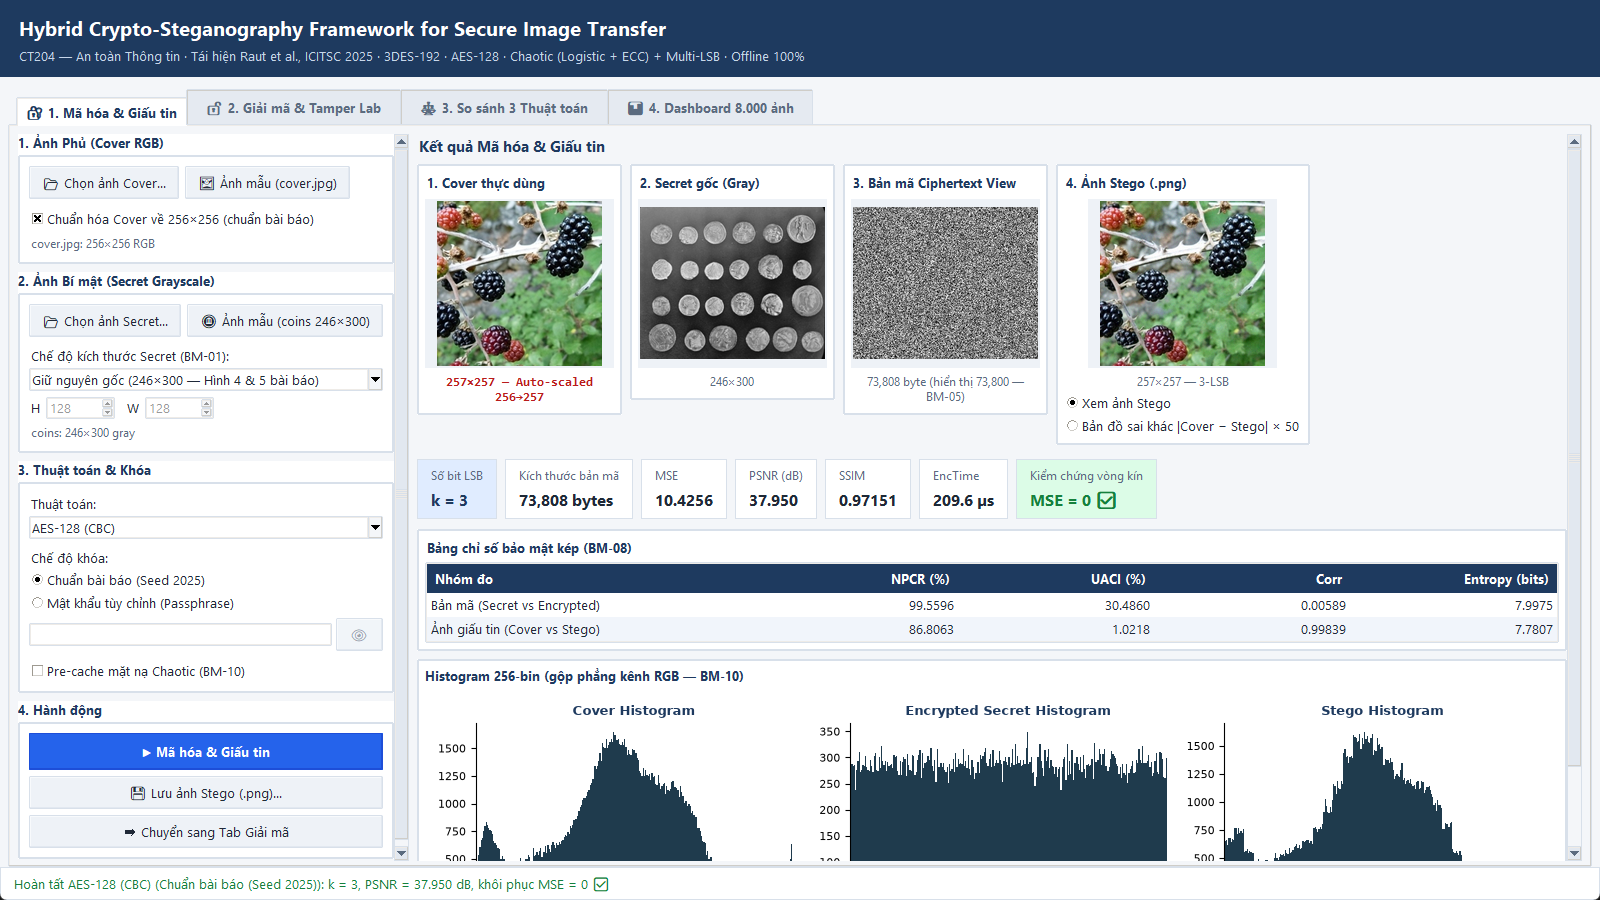
\includegraphics[width=\linewidth]{tab1_encrypt}
\caption{Tab 1 -- mã hóa AES-128 và giấu ảnh $246\times300$ (tự động chọn 3-LSB và phóng to ảnh
phủ lên $257\times257$)}
\label{fig:ui-tab1}
\end{figure}

\subsection{Tab 2 -- Giải mã và phòng thí nghiệm tấn công}

Tab 2 mô phỏng phía nhận: mở một ảnh stego bất kỳ (hoặc nhận trực tiếp từ Tab 1), đọc và hiển thị
từng trường của header kèm trạng thái kiểm tra CRC, rồi trích xuất và giải mã. Phần ``phòng thí
nghiệm tấn công'' (\tn{tamper lab}) cho phép áp dụng năm kịch bản lên ảnh stego: giải mã bằng sai
khóa, nén JPEG chất lượng 95, đảo một bit trong header, đảo 1\% bit LSB của vùng dữ liệu và cộng
nhiễu Gauss $\sigma = 2$. Hệ thống báo rõ quá trình dừng ở giai đoạn nào (header, trích xuất hay
giải mã) và vì sao (\hinh{fig:ui-tab2}).

\begin{figure}[H]
\centering
\begin{subfigure}{\linewidth}
  \centering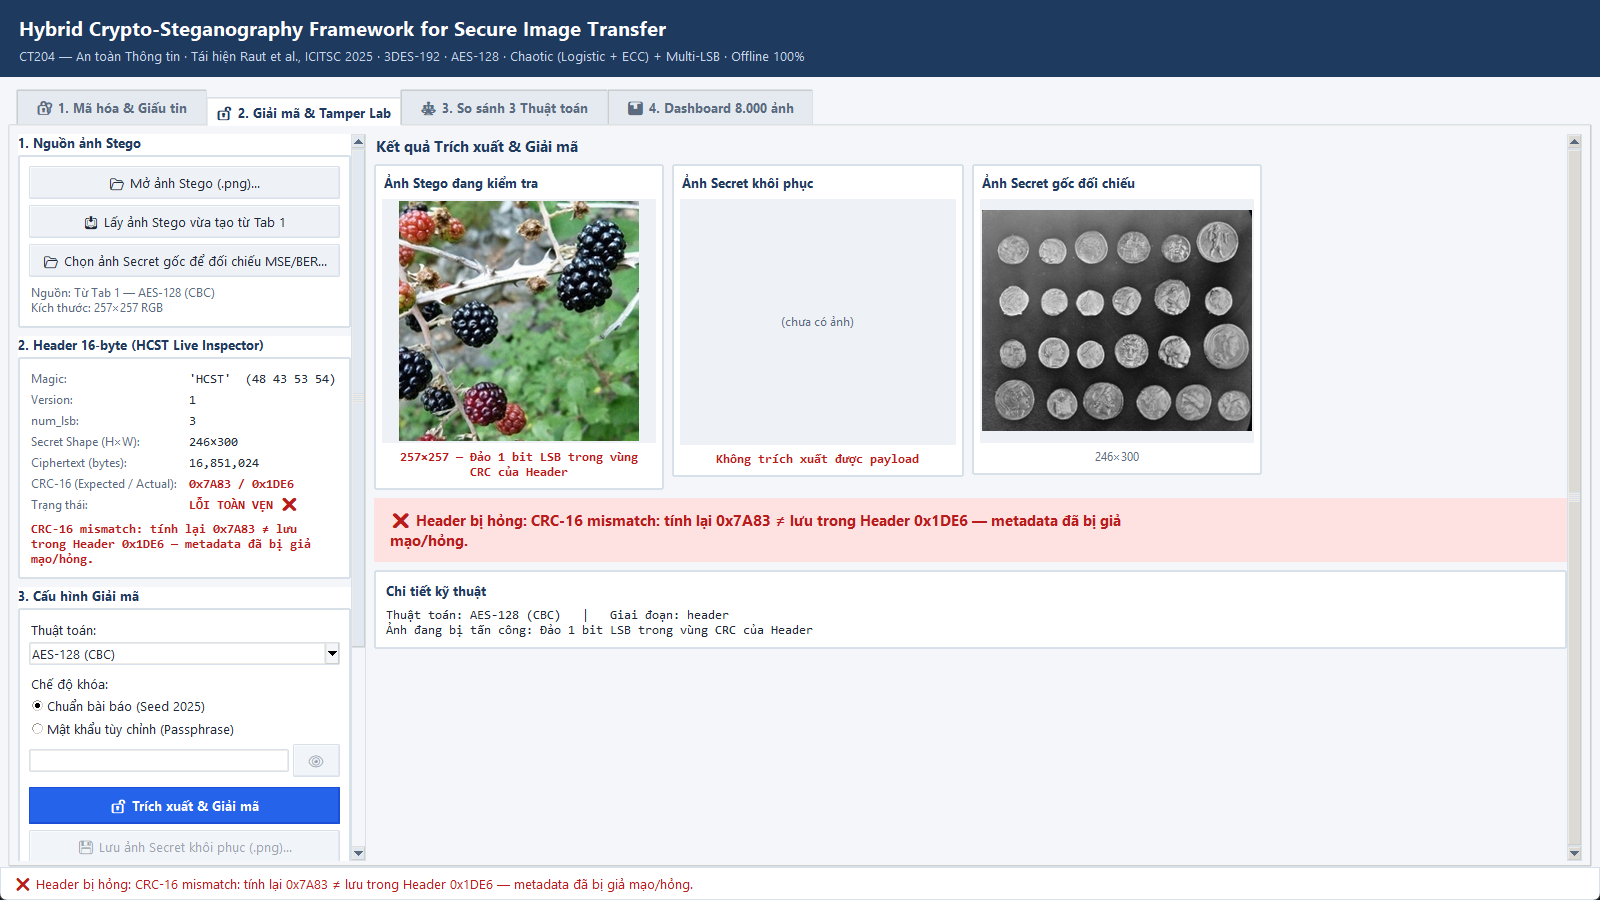
\includegraphics[width=0.93\linewidth]{tab2_tamper}
  \caption{Đảo 1 bit trong trường \code{ciphertext\_len}: magic vẫn đúng nhưng CRC-16 phát hiện
  header bị sửa}
\end{subfigure}

\vspace{3mm}
\begin{subfigure}{\linewidth}
  \centering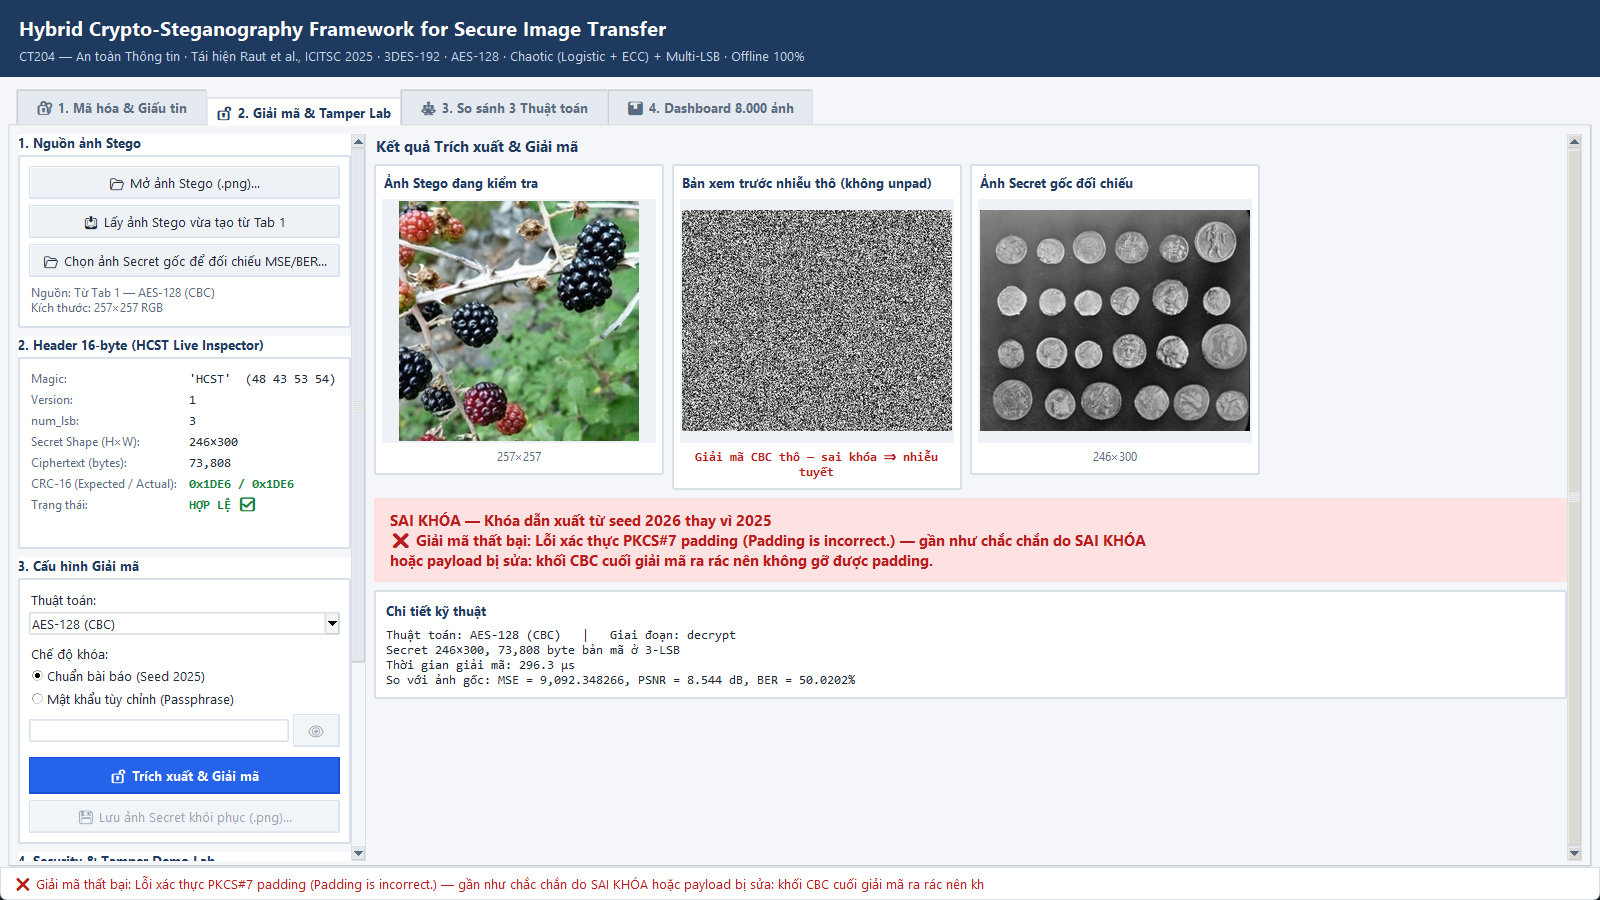
\includegraphics[width=0.93\linewidth]{tab2_wrongkey}
  \caption{Giải mã AES bằng khóa sai: lỗi gỡ đệm PKCS\#7, hiển thị dữ liệu giải mã thô (nhiễu)}
\end{subfigure}
\caption{Tab 2 -- kiểm tra header và phòng thí nghiệm tấn công}
\label{fig:ui-tab2}
\end{figure}

\subsection{Tab 3 -- So sánh ba thuật toán}

Tab 3 chạy cả ba thuật toán trên cùng một cặp ảnh và dựng lại Hình~5 của bài báo (ảnh mã hóa,
histogram bản mã, histogram ảnh stego của từng thuật toán), kèm bảng so sánh đầy đủ các độ đo và hệ
số tăng tốc so với 3DES (\hinh{fig:ui-tab3}). Toàn bộ kết quả có thể xuất ra thư mục dưới dạng ảnh
PNG và tệp CSV.

\begin{figure}[H]
\centering
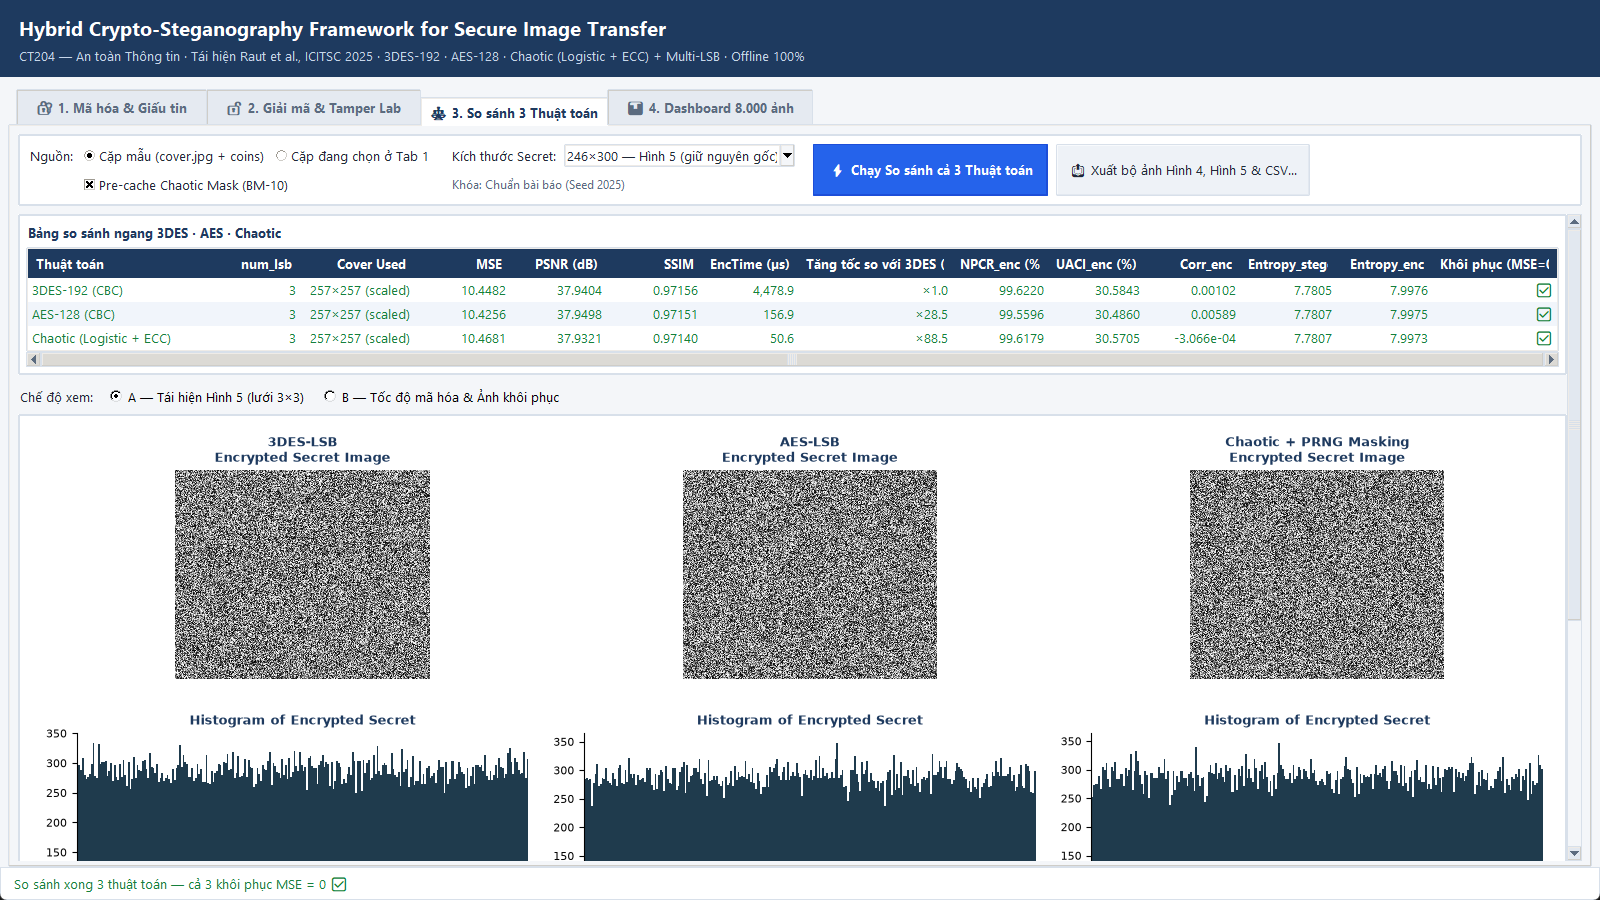
\includegraphics[width=\linewidth]{tab3_compare}
\caption{Tab 3 -- so sánh 3DES, AES và Chaotic trên cùng một cặp ảnh}
\label{fig:ui-tab3}
\end{figure}

\subsection{Tab 4 -- Bảng điều khiển kết quả 8000 ảnh}

Tab 4 nạp hai tệp CSV kết quả benchmark, hiển thị bảng đối chiếu ``Python -- bài báo -- chênh lệch''
cho từng thuật toán và các biểu đồ có thể lọc theo tập dữ liệu (\code{train}/\code{test}) và theo
lớp ảnh (\hinh{fig:ui-tab4}).

\begin{figure}[H]
\centering
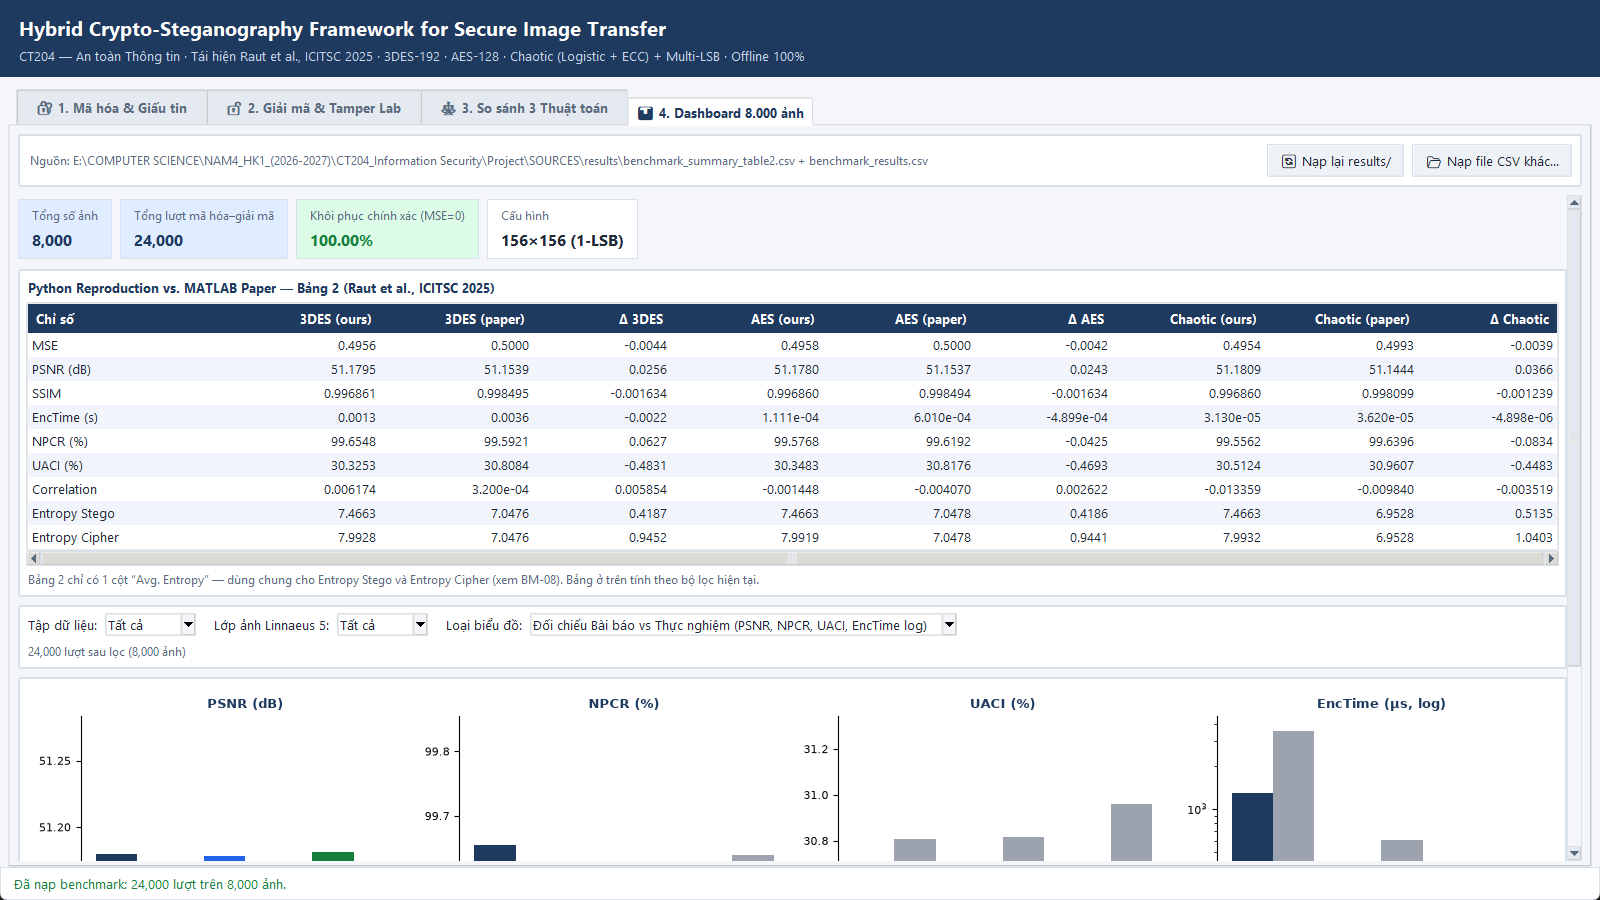
\includegraphics[width=\linewidth]{tab4_benchmark}
\caption{Tab 4 -- bảng điều khiển đối chiếu kết quả 8000 ảnh với Bảng~2 của bài báo}
\label{fig:ui-tab4}
\end{figure}

\subsection{Đóng gói thành tệp thực thi}

Ứng dụng được đóng gói bằng PyInstaller ở chế độ \emph{onedir} (\code{packaging/ct204\_app.spec}),
cho ra thư mục \code{CT204\_CryptoStego} gồm tệp \code{CT204\_CryptoStego.exe} và thư mục
\code{\_internal}. Gói kèm tệp cấu hình, cặp ảnh mẫu và các tệp kết quả benchmark, nhưng không kèm
8000 ảnh gốc. Khi chạy dạng \code{.exe}, ứng dụng tự xác định thư mục tài nguyên qua biến
\code{sys.\_MEIPASS} và chuyển bộ nhớ đệm JIT của Numba sang thư mục tạm để tránh lỗi ghi vào thư
mục chương trình. Người dùng chỉ cần giải nén và chạy, không cần cài Python.

\section{Kiểm thử phần mềm}

Hệ thống được kiểm thử tự động bằng pytest với tổng cộng \textbf{347 ca kiểm thử}
(\bang{tab:tests}). Toàn bộ 347 ca đều đạt khi chạy trên môi trường ở \bang{tab:tech}. Các ca kiểm
thử quan trọng nhất là kiểm thử khứ hồi (\tn{round-trip}): với mọi thuật toán, mọi kích thước ảnh
(kể cả ảnh toàn 0, ảnh có kích thước là bội số của 8/16, ảnh lớn buộc phải phóng to ảnh phủ), ảnh
khôi phục phải giống hệt ảnh gốc.

\begin{table}[H]
\centering
\caption{Thống kê các ca kiểm thử tự động}
\label{tab:tests}
\small
\begin{tabularx}{\linewidth}{@{}P{4.6cm}rL@{}}
\toprule
\thead{Tệp kiểm thử} & \thead{Số ca} & \thead{Nội dung chính}\\
\midrule
\code{test\_crypto.py}   & 126 & Khứ hồi cả 3 thuật toán; độ dài khóa/IV; đệm PKCS\#7; tính tất định; khóa 3DES suy biến; JIT warm-up; chế độ cache mặt nạ\\
\code{test\_lsb.py}      & 71  & Đóng gói/kiểm tra header, CRC; chọn $k$; công thức phóng to; nhúng/trích khứ hồi; phát hiện ảnh hỏng; không có vòng lặp Python trên điểm ảnh\\
\code{test\_metrics.py}  & 38  & MSE, PSNR, SSIM, NPCR, UACI, entropy, tương quan trên các ca đã biết đáp án; đo EncTime; chạy thử hai kịch bản \code{run\_single}, \code{run\_benchmark}\\
\code{test\_pipeline.py} & 40  & Đầu -- cuối: ảnh khôi phục giống hệt (MSE $=0$); ghi/đọc PNG; từ chối lưu JPEG\\
\code{test\_ui\_controller.py} & 72 & Nghiệp vụ giao diện: hai chế độ khóa, kiểm tra header, 4 kịch bản tấn công, xuất kết quả, luồng nền, chạy thử toàn bộ giao diện\\
\midrule
\textbf{Tổng} & \textbf{347} & \textbf{Tất cả đều đạt}\\
\bottomrule
\end{tabularx}
\end{table}

% =====================================================================
%  Chương 3 (tiếp) — Kết quả thực nghiệm và phân tích an toàn mở rộng
% =====================================================================

\section{Kết quả thực nghiệm}
\label{sec:ketqua}

\subsection{Dữ liệu, môi trường và kịch bản thực nghiệm}

Ảnh phủ là toàn bộ 8000 ảnh của bộ dữ liệu Linnaeus 5 \cite{chaladze2017}, gồm 5 lớp
(\hinh{fig:linnaeus}), mỗi lớp 1200 ảnh huấn luyện và 400 ảnh kiểm tra, kích thước $256\times256$.
Ảnh bí mật là ảnh xám ``coins'', lấy từ \code{skimage.data.coins()} và chuẩn hóa về kích thước
\code{coins.png} của MATLAB ($246\times300$) bằng nội suy \code{INTER\_AREA}. Cấu hình máy chạy thực
nghiệm được nêu ở \bang{tab:env}.

\begin{figure}[H]
\centering
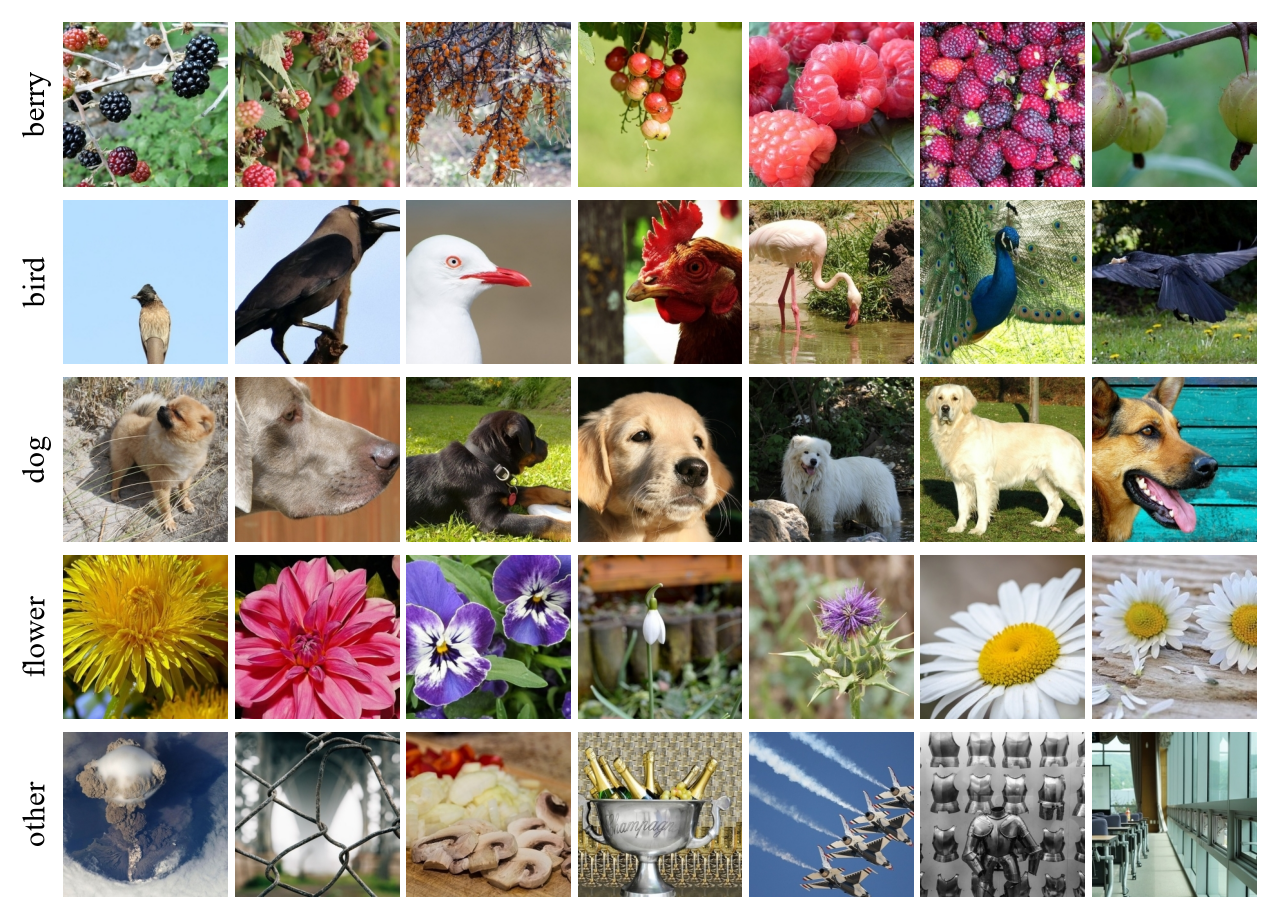
\includegraphics[width=0.86\linewidth]{linnaeus5_samples}
\caption{Một số ảnh phủ của bộ dữ liệu Linnaeus 5 (mỗi hàng là một lớp)}
\label{fig:linnaeus}
\end{figure}

\begin{table}[H]
\centering
\caption{Môi trường thực nghiệm}
\label{tab:env}
\small
\begin{tabularx}{0.85\linewidth}{@{}P{3.6cm}L@{}}
\toprule
\thead{Thành phần} & \thead{Cấu hình}\\
\midrule
Bộ xử lý & Intel Core i3-1005G1 (2 nhân, 4 luồng, xung cơ bản 1.20 GHz, hỗ trợ AES-NI)\\
Bộ nhớ & 20 GB RAM\\
Hệ điều hành & Windows 11 IoT Enterprise LTSC 2024 (64 bit)\\
Phần mềm & Python 3.12.8 và các thư viện ở \bang{tab:tech}\\
\bottomrule
\end{tabularx}
\end{table}

Theo quyết định BM-01, thực nghiệm được tổ chức thành hai kịch bản bổ sung cho nhau
(\bang{tab:scenarios}).

\begin{table}[H]
\centering
\caption{Hai kịch bản thực nghiệm}
\label{tab:scenarios}
\small
\begin{tabularx}{\linewidth}{@{}P{3.2cm}LL@{}}
\toprule
\thead{Thuộc tính} & \thead{Kịch bản A -- một cặp ảnh} & \thead{Kịch bản B -- benchmark}\\
\midrule
Mục đích & Tái hiện Hình~4 và Hình~5 & Tái hiện Bảng~2\\
Ảnh phủ & Ảnh mẫu \code{berry} & 8000 ảnh Linnaeus 5\\
Ảnh bí mật & $246\times300$ (\num{73800} byte) & $156\times156$ (\num{24336} byte)\\
Số bit LSB & 3 (ảnh phủ phóng to lên $257\times257$) & 1 (không phóng to)\\
Số lượt chạy & 3 (một lượt mỗi thuật toán) & \num{24000} ($8000 \times 3$)\\
Chaotic khi đo EncTime & Sinh lại mặt nạ mỗi lần & Cache mặt nạ (\code{--cache-chaotic-mask})\\
Kịch bản dòng lệnh & \code{scripts.run\_single} & \code{scripts.run\_benchmark --secret-size 156 156}\\
\bottomrule
\end{tabularx}
\end{table}

\subsection{Kết quả trên một cặp ảnh mẫu}

\hinh{fig:fig4} và \hinh{fig:fig5} là kết quả tái hiện Hình~4 và Hình~5 của bài báo. Histogram
ảnh phủ và ảnh bí mật (\hinh{fig:fig4}) có hình dạng tương tự bài báo: ảnh phủ có một đỉnh lớn
quanh mức 100--130, còn ảnh ``coins'' tập trung ở vùng tối 30--60 do nền ảnh. Ở \hinh{fig:fig5},
bản mã của cả ba thuật toán trông như nhiễu ngẫu nhiên, histogram phẳng với khoảng 288 điểm ảnh
mỗi mức, và histogram ảnh stego giữ nguyên hình dạng histogram ảnh phủ.

\begin{figure}[H]
\centering
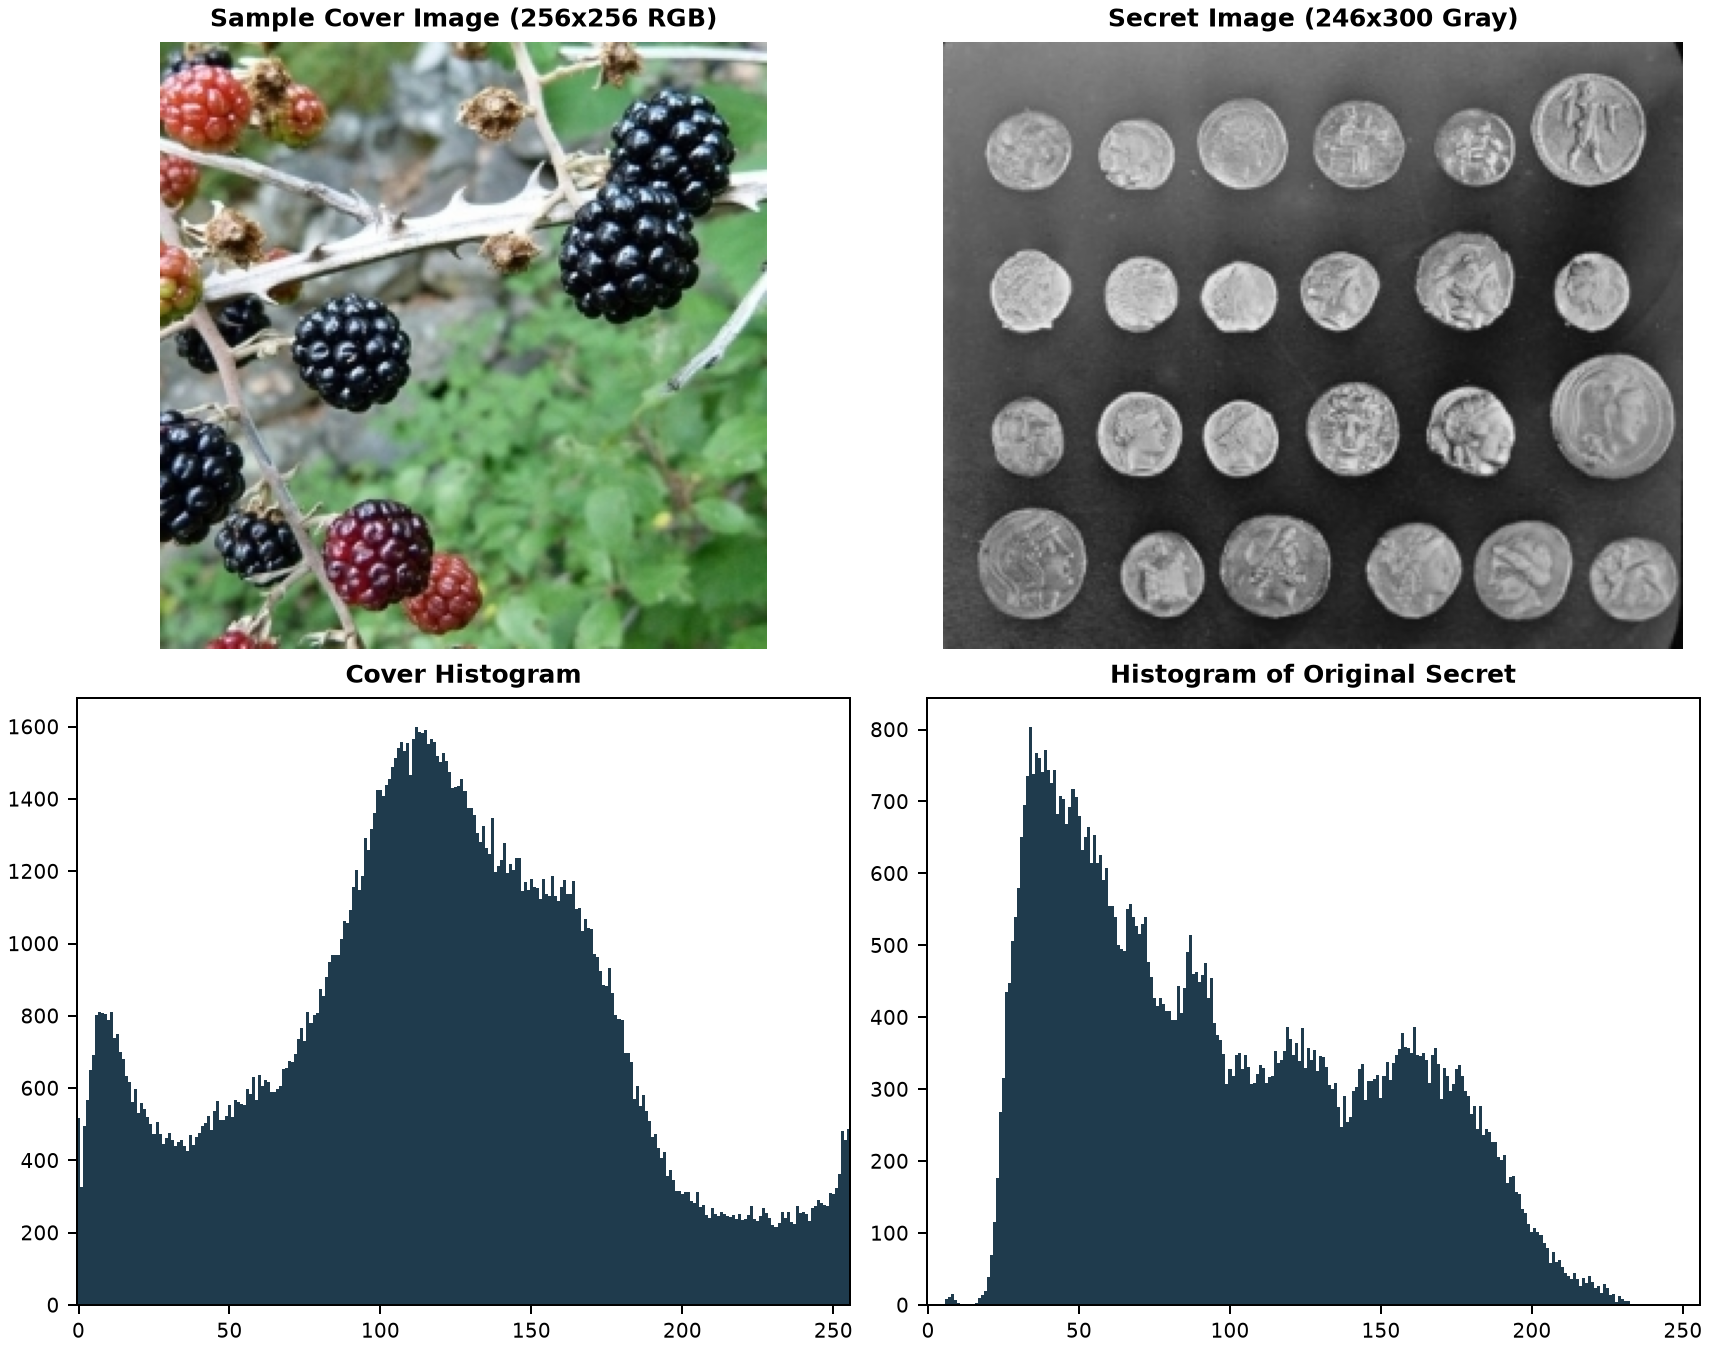
\includegraphics[width=0.82\linewidth]{fig4_cover_secret_histograms}
\caption{Tái hiện Hình~4 của bài báo: ảnh phủ, ảnh bí mật và histogram tương ứng}
\label{fig:fig4}
\end{figure}

\begin{figure}[H]
\centering
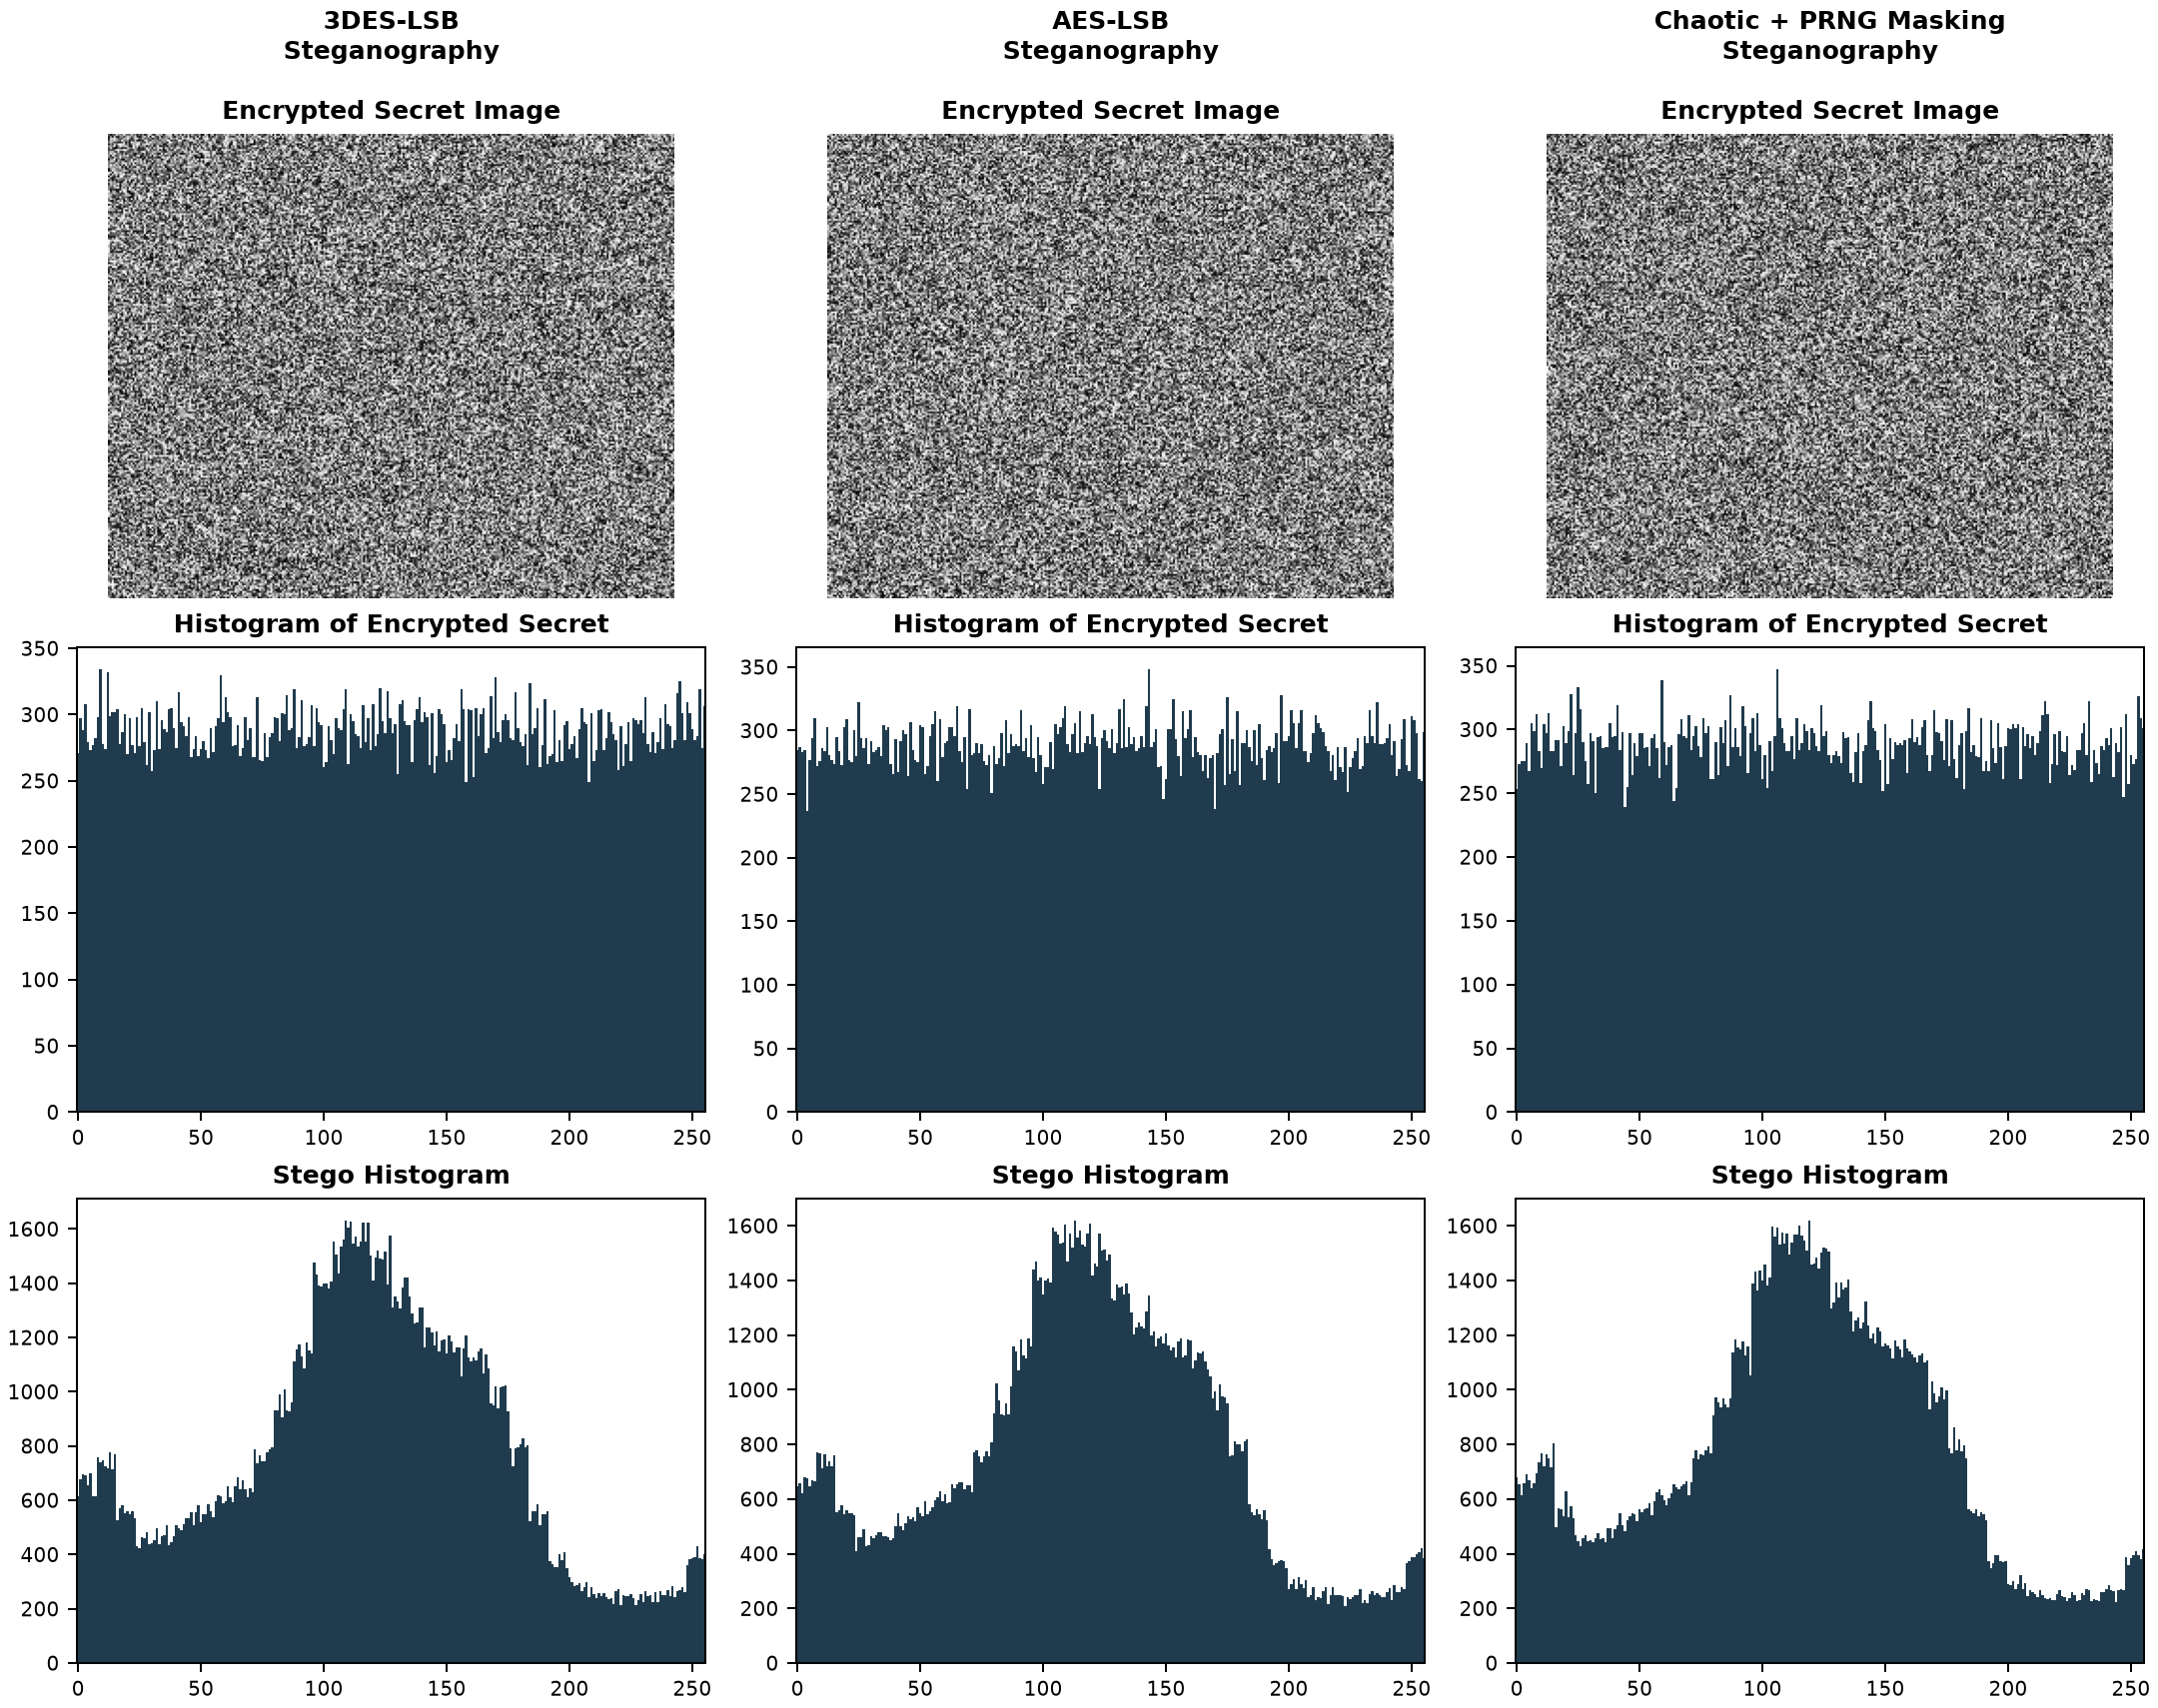
\includegraphics[width=0.92\linewidth]{fig5_comparison_grid}
\caption{Tái hiện Hình~5 của bài báo: bản mã, histogram bản mã và histogram ảnh stego của
3DES-LSB, AES-LSB và Chaotic-LSB (ảnh bí mật $246\times300$)}
\label{fig:fig5}
\end{figure}

\bang{tab:single} trình bày các độ đo của kịch bản A. Cả ba thuật toán đều khôi phục ảnh bí mật
chính xác tuyệt đối. Do tải tin \num{73800} byte vượt dung lượng 3-LSB của ảnh $256\times256$, hệ
thống tự động chọn $k = 3$ và phóng to ảnh phủ lên $257\times257$. MSE đo được ($\approx 10.43$)
khớp với giá trị lý thuyết $10.5\times99.3\%$ suy ra từ \pt{eq:lsb-mse}, trong đó $99.3\%$ là tỷ lệ
kênh màu thực sự được dùng. PSNR \SI{37.94}{dB} vẫn đủ cao để mắt thường không phân biệt được.

\begin{table}[H]
\centering
\caption{Kết quả kịch bản A -- ảnh bí mật $246\times300$, 3-LSB, ảnh phủ $257\times257$}
\label{tab:single}
\small
\begin{tabular}{@{}lrrr@{}}
\toprule
\thead{Độ đo} & \thead{3DES} & \thead{AES-128} & \thead{Chaotic}\\
\midrule
Độ dài bản mã (byte) & \num{73808} & \num{73808} & \num{73800}\\
MSE / PSNR (dB) & 10.448 / 37.94 & 10.426 / 37.95 & 10.468 / 37.93\\
SSIM & 0.97156 & 0.97151 & 0.97140\\
EncTime ($\mu$s) & \num{3587.7} & 285.1 & 834.5\\
NPCR\textsubscript{enc} / UACI\textsubscript{enc} (\%) & 99.622 / 30.584 & 99.560 / 30.486 & 99.618 / 30.570\\
Entropy bản mã (bit) & 7.99760 & 7.99751 & 7.99727\\
Khôi phục chính xác (MSE $= 0$) & \ok & \ok & \ok\\
\bottomrule
\end{tabular}
\end{table}

\hinh{fig:distortion} so sánh độ méo do nhúng ở hai mức tải tin. Ở 1-LSB, mỗi giá trị kênh thay đổi
nhiều nhất 1 đơn vị và chỉ $49.5\%$ số giá trị bị thay đổi (vì một nửa số bit nhúng tình cờ trùng
bit gốc). Ở 3-LSB, độ lệch tối đa là 7 và $86.8\%$ số giá trị bị thay đổi. Trong cả hai trường hợp,
bản đồ sai khác (đã khuếch đại) đều là nhiễu đều, không lộ đường nét của ảnh bí mật, nhờ bản mã có
phân bố bit ngẫu nhiên.

\begin{figure}[H]
\centering
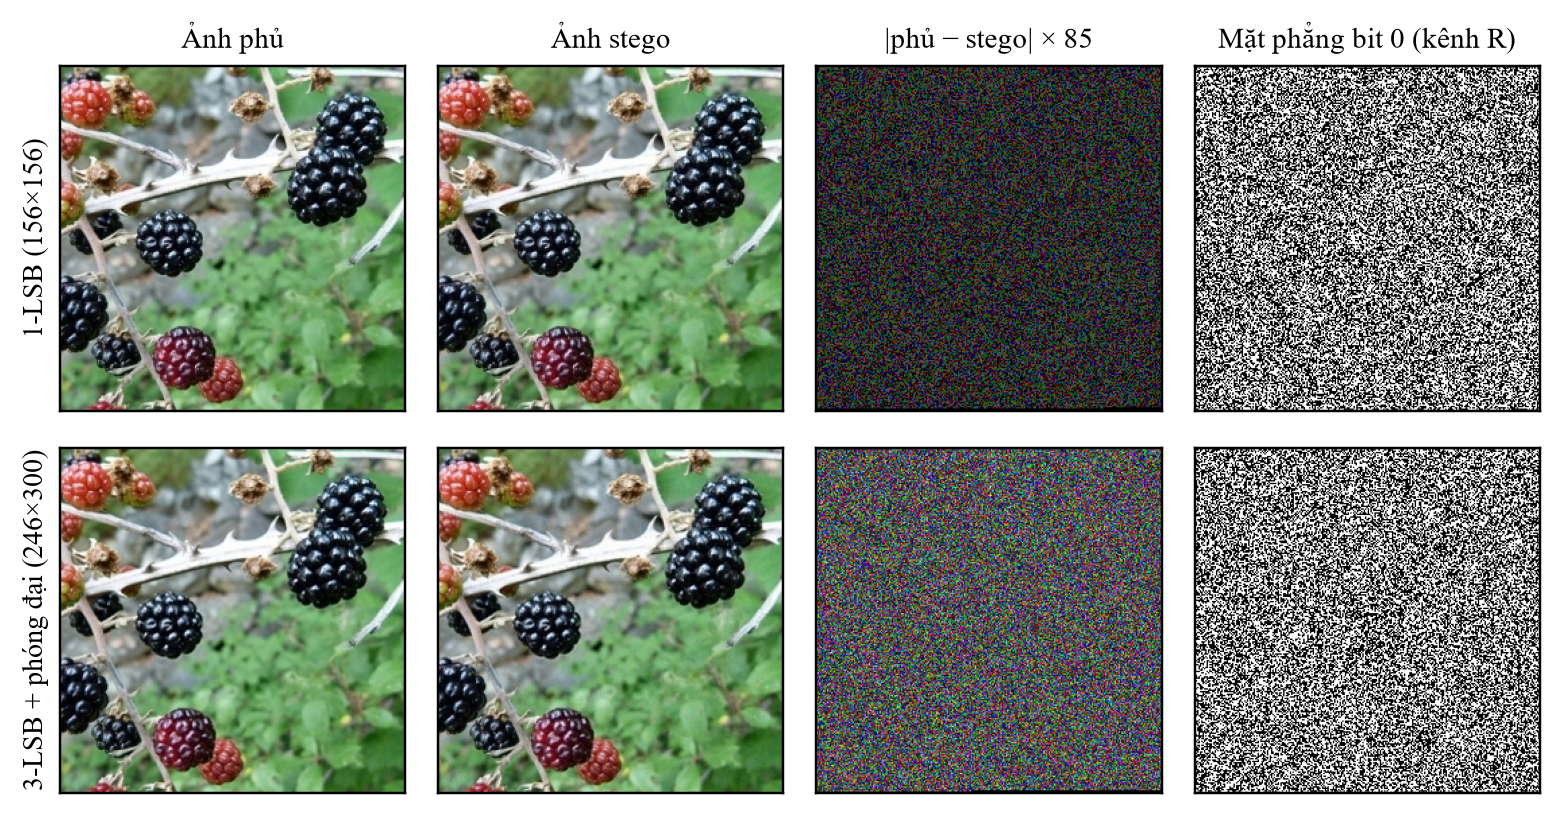
\includegraphics[width=\linewidth]{embedding_distortion}
\caption{Độ méo do nhúng: ảnh phủ, ảnh stego, sai khác tuyệt đối đã khuếch đại và mặt phẳng bit
thấp nhất (kênh R) ở hai mức tải tin}
\label{fig:distortion}
\end{figure}

\subsection{Chất lượng thị giác trên 8000 ảnh}

Ở kịch bản B, bản mã \num{24336}--\num{24352} byte cùng 128 bit header chiếm
$(128 + 8\cdot\num{24336}) / (3\cdot256^2) = 99.09\%$ số giá trị kênh. Theo \pt{eq:lsb-mse}, giá trị
kỳ vọng của MSE là $0.5\times0.9909 = 0.4954$, tương ứng PSNR $= \SI{51.18}{dB}$. Kết quả thực nghiệm
(\bang{tab:visual}, \hinh{fig:visual}) khớp gần như tuyệt đối với giá trị lý thuyết này. Toàn bộ
\num{24000} lượt chạy đều khôi phục ảnh bí mật chính xác và đều dùng 1-LSB.

\begin{table}[H]
\centering
\caption{Chất lượng thị giác trung bình trên 8000 ảnh (độ lệch chuẩn trong ngoặc)}
\label{tab:visual}
\small
\begin{tabular}{@{}llll@{}}
\toprule
\thead{Thuật toán} & \thead{MSE} & \thead{PSNR (dB)} & \thead{SSIM}\\
\midrule
3DES -- bài báo   & 0.499975 & 51.15389 & 0.998495\\
3DES -- tái hiện  & 0.495602 (0.0011) & 51.17948 (0.0099) & 0.996861 (0.0019)\\
AES -- bài báo    & 0.500006 & 51.15373 & 0.998494\\
AES -- tái hiện   & 0.495773 (0.0011) & 51.17798 (0.0098) & 0.996860 (0.0019)\\
Chaotic -- bài báo & 0.499321 & 51.14436 & 0.998099\\
Chaotic -- tái hiện & 0.495439 (0.0011) & 51.18092 (0.0097) & 0.996860 (0.0019)\\
\midrule
Lý thuyết (tải 99.09\%) & 0.4954 & 51.18 & --\\
\bottomrule
\end{tabular}
\end{table}

\begin{figure}[H]
\centering
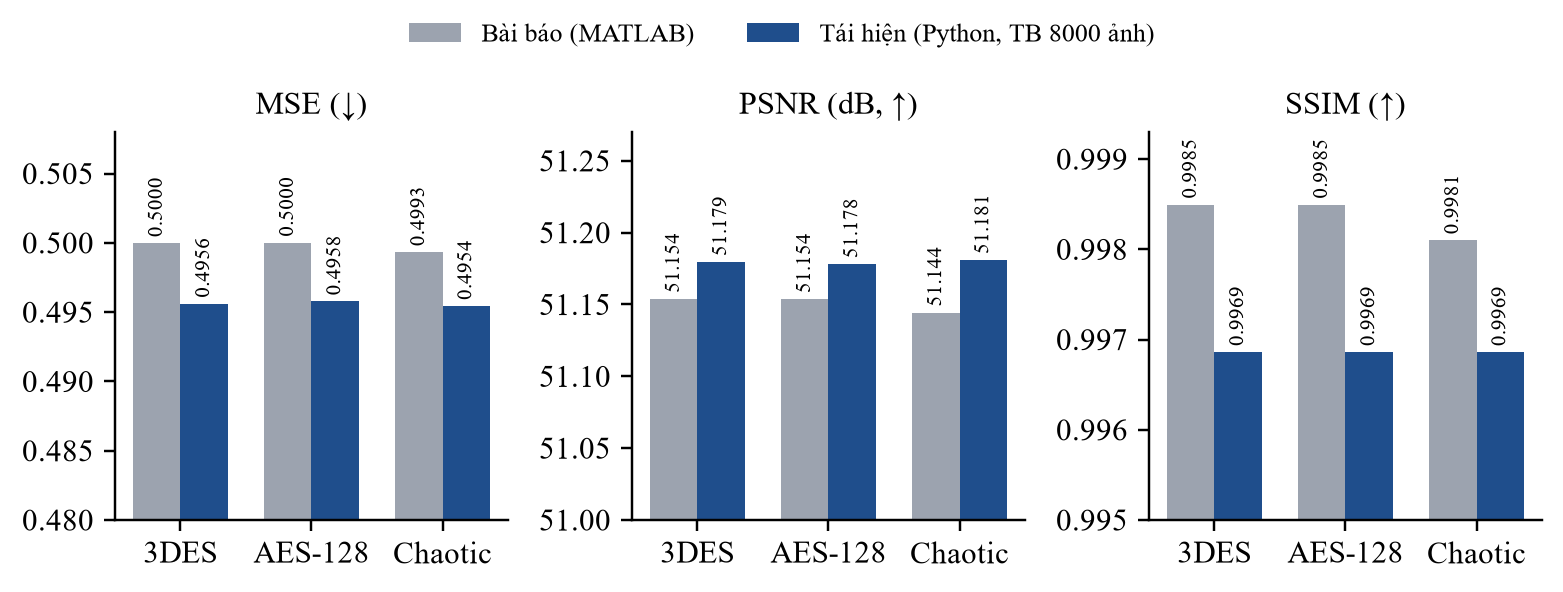
\includegraphics[width=\linewidth]{visual_paper_vs_ours}
\caption{So sánh MSE, PSNR, SSIM trung bình giữa bài báo và kết quả tái hiện}
\label{fig:visual}
\end{figure}

\begin{figure}[H]
\centering
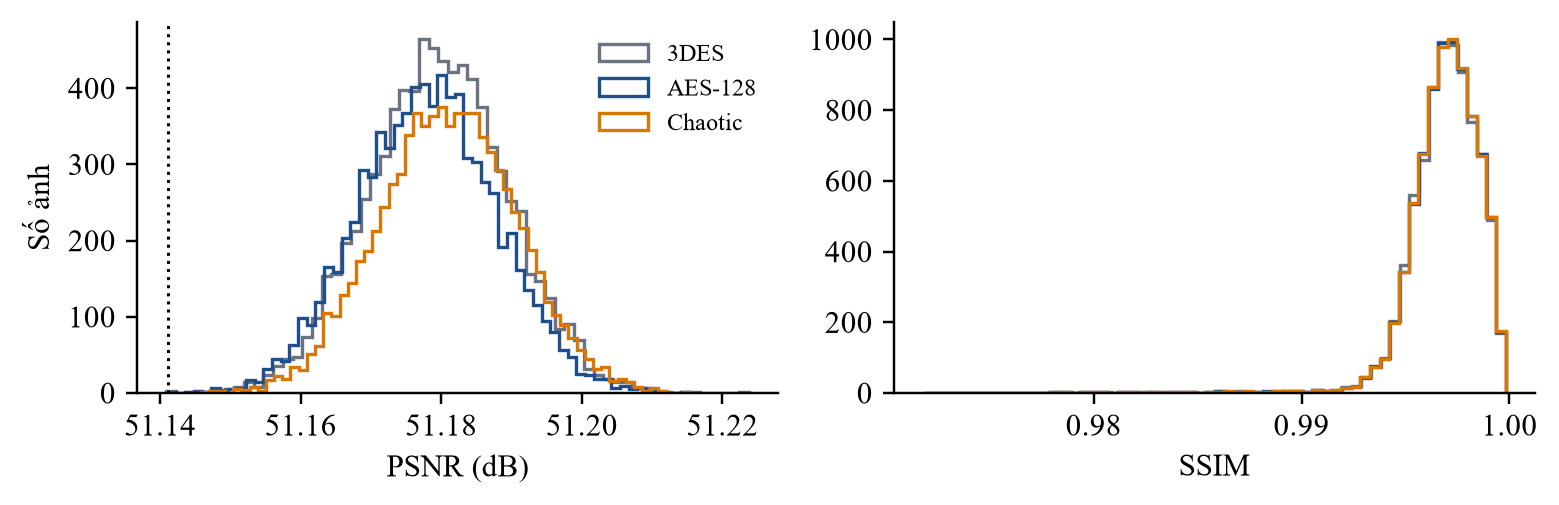
\includegraphics[width=\linewidth]{psnr_ssim_distribution}
\caption{Phân bố PSNR và SSIM trên 8000 ảnh (đường chấm: PSNR lý thuyết khi lấp đầy 100\% 1-LSB)}
\label{fig:psnr-dist}
\end{figure}

Nhận xét:
\begin{itemize}
  \item MSE và PSNR lệch bài báo dưới $1\%$ (PSNR lệch khoảng \SI{0.03}{dB}). Chênh lệch nhỏ này
        hoàn toàn do tỷ lệ lấp đầy: bài báo có MSE $\approx 0.5000$, tức đã lấp gần $100\%$ dung
        lượng 1-LSB, trong khi ảnh $156\times156$ lấp $99.09\%$.
  \item PSNR dao động rất hẹp (\SIrange{51.14}{51.22}{dB}) và gần như không phụ thuộc nội dung ảnh
        phủ hay thuật toán mã hóa, đúng như dự đoán từ \pt{eq:lsb-mse}: khi bit nhúng là ngẫu
        nhiên, độ méo chỉ phụ thuộc số bit nhúng.
  \item SSIM trung bình thấp hơn bài báo khoảng $0.0016$. Trên ảnh phủ đầu tiên (\code{berry}),
        SSIM đạt $0.99855$, gần như trùng giá trị $0.998495$ của bài báo; nhưng trên toàn bộ dữ liệu,
        các ảnh có vùng nền phẳng lớn (bầu trời, phông mờ) có SSIM thấp tới $0.972$ và kéo trung bình
        xuống. Bài báo không công bố cách tính SSIM cho ảnh màu nên không thể xác định chính xác
        nguyên nhân chênh lệch này.
\end{itemize}

\subsection{Độ an toàn thống kê của bản mã}
\label{sec:ketqua-antoan}

\bang{tab:enc-metrics} và \hinh{fig:dual} trình bày hai nhóm độ đo an toàn theo quyết định BM-08.
Một điểm quan trọng: vì khóa cố định và ảnh bí mật không đổi, bản mã của mỗi thuật toán \emph{giống
hệt nhau} trên cả 8000 lượt. Do đó các độ đo nhóm \code{*\_enc} thực chất là giá trị của một bản mã
duy nhất. Khác biệt NPCR giữa các thuật toán (ví dụ $99.59\%$ so với $99.64\%$ trong bài báo) chỉ là
dao động thống kê của một mẫu, không phản ánh thuật toán nào ``tốt hơn''.

\begin{table}[H]
\centering
\caption{Hai nhóm độ đo an toàn trung bình trên 8000 ảnh (ảnh bí mật $156\times156$)}
\label{tab:enc-metrics}
\small
\begin{tabular}{@{}lrrrr@{}}
\toprule
\thead{Độ đo} & \thead{3DES} & \thead{AES-128} & \thead{Chaotic} & \thead{Bài báo (AES)}\\
\midrule
\multicolumn{5}{@{}l}{\textit{Nhóm bản mã (ảnh bí mật -- bản mã)}}\\
NPCR\textsubscript{enc} (\%)    & 99.6548 & 99.5768 & 99.5562 & 99.6192\\
UACI\textsubscript{enc} (\%)    & 30.3253 & 30.3483 & 30.5124 & 30.8176\\
Tương quan\textsubscript{enc}   & 0.00617 & $-0.00145$ & $-0.01336$ & $-0.00407$\\
Entropy bản mã (bit)            & 7.99285 & 7.99189 & 7.99318 & --\\
\midrule
\multicolumn{5}{@{}l}{\textit{Nhóm ảnh stego (ảnh phủ -- ảnh stego)}}\\
NPCR\textsubscript{stego} (\%)  & 49.560 & 49.577 & 49.544 & --\\
UACI\textsubscript{stego} (\%)  & 0.1944 & 0.1944 & 0.1943 & --\\
Tương quan\textsubscript{stego} & 0.99989 & 0.99989 & 0.99989 & --\\
Entropy ảnh stego (bit)         & 7.46633 & 7.46633 & 7.46634 & 7.04776\\
\bottomrule
\end{tabular}
\end{table}

\begin{figure}[H]
\centering
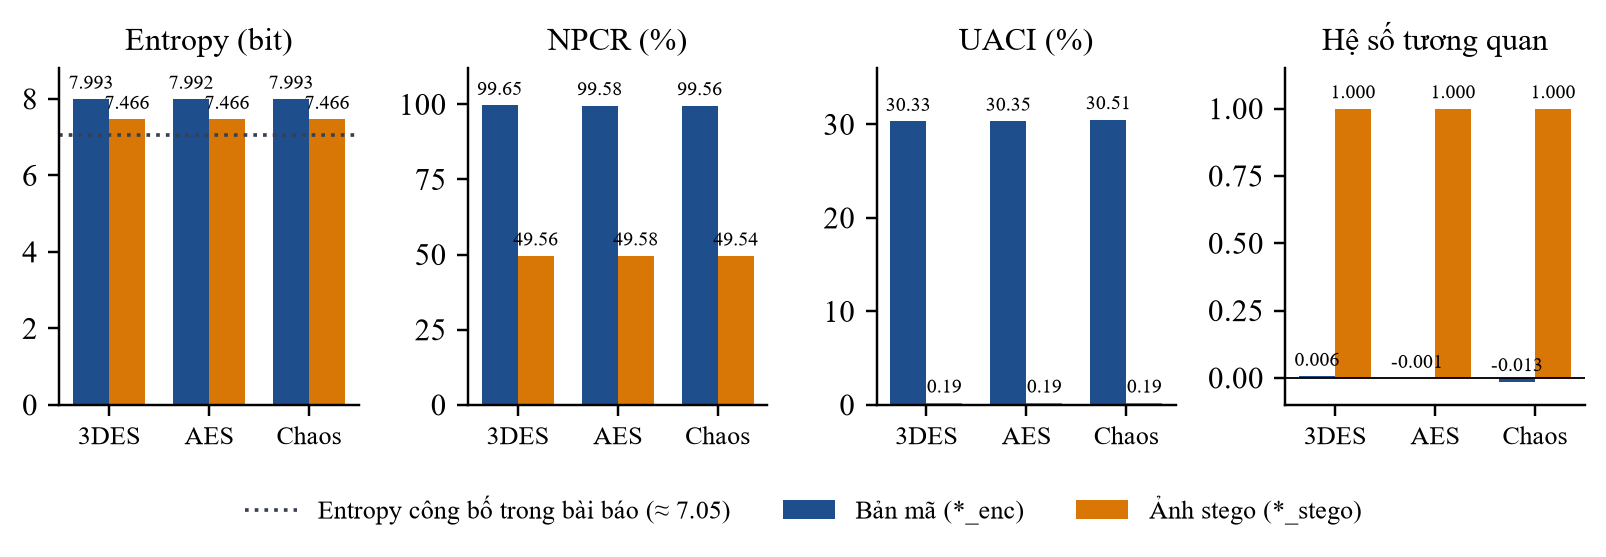
\includegraphics[width=\linewidth]{dual_metrics}
\caption{Hai nhóm độ đo: bản mã (\code{*\_enc}) và ảnh stego (\code{*\_stego})}
\label{fig:dual}
\end{figure}

Từ kết quả trên có thể giải thích đầy đủ các con số an toàn trong Bảng~2 của bài báo:
\begin{itemize}
  \item \textbf{NPCR} của cả ba thuật toán xấp xỉ giá trị lý thuyết $255/256 = 99.609\%$ của một
        bản mã ngẫu nhiên đều.
  \item \textbf{UACI} $\approx 30.3$--$30.5\%$, thấp hơn ngưỡng $33.46\%$ mà bài báo nêu. Đây
        \emph{không} phải dấu hiệu bản mã yếu. Khi so một ảnh bí mật cố định với một bản mã ngẫu
        nhiên đều $U$, giá trị kỳ vọng của UACI bằng
        $\frac{1}{mn}\sum_{i,j}\mathbb{E}\,|I(i,j) - U| / 255$ và phụ thuộc phân bố mức xám của
        ảnh bí mật. Tính trực tiếp trên ảnh ``coins'' $156\times156$ (độ sáng trung bình 96.9) cho
        giá trị kỳ vọng $30.41\%$, khớp với thực nghiệm. Ngưỡng $33.46\%$ chỉ đúng khi so hai ảnh
        ngẫu nhiên đều với nhau.
  \item \textbf{Entropy}: bản mã của cả ba thuật toán có entropy $\approx 7.992$--$7.993$ bit, sát
        cực đại 8. Giá trị $\approx 7.05$ trong bài báo nằm trong khoảng entropy của ảnh stego (ảnh
        màu tự nhiên, ở đây trung bình $7.47$), chứng tỏ bài báo đo entropy trên ảnh stego chứ
        không phải trên bản mã. Entropy của ảnh stego gần như bằng entropy của ảnh phủ và hầu như
        không phụ thuộc thuật toán mã hóa. Vì vậy kết luận của bài báo rằng Chaotic ``có entropy
        thấp hơn, cần nghiên cứu thêm về tính ngẫu nhiên'' không có cơ sở.
  \item \textbf{Tương quan} giữa ảnh bí mật và bản mã xấp xỉ 0 ở cả ba thuật toán, trong khi tương
        quan giữa ảnh phủ và ảnh stego là $0.9999$, phản ánh đúng vai trò của hai lớp: lớp mã hóa
        phá vỡ mọi liên hệ với bản rõ, lớp giấu tin giữ ảnh mang tin gần như không đổi.
\end{itemize}

Để đánh giá kỹ hơn tính ngẫu nhiên, em tính thêm tương quan giữa các điểm ảnh kề nhau và kiểm định
$\chi^2$ tính đều của histogram ($\chi^2 = \sum_i (o_i - e_i)^2/e_i$ với 255 bậc tự do, giá trị
tới hạn ở mức ý nghĩa $5\%$ là $293.25$). Kết quả ở \bang{tab:adjacent} và \hinh{fig:scatter} cho
thấy ảnh bí mật có tương quan điểm ảnh kề rất cao (0.89--0.94), còn bản mã của cả ba thuật toán có
tương quan xấp xỉ 0 và đều vượt qua kiểm định tính đều.

\begin{table}[H]
\centering
\caption{Tương quan điểm ảnh kề, entropy và kiểm định $\chi^2$ tính đều ($156\times156$)}
\label{tab:adjacent}
\small
\begin{tabular}{@{}lrrrrrc@{}}
\toprule
\thead{Ảnh} & \thead{Ngang} & \thead{Dọc} & \thead{Chéo} & \thead{Entropy} & \thead{$\chi^2$} & \thead{Đều?}\\
\midrule
Ảnh bí mật       & 0.92566 & 0.94084 & 0.88696 & 7.4252 & \num{15143.5} & \no\\
Bản mã 3DES      & $-0.00255$ & 0.00860 & 0.00398 & 7.9928 & 241.2 & \ok\\
Bản mã AES-128   & $-0.00565$ & $-0.00265$ & 0.01160 & 7.9919 & 272.3 & \ok\\
Bản mã Chaotic   & $-0.00211$ & 0.00702 & 0.00050 & 7.9932 & 231.9 & \ok\\
\bottomrule
\end{tabular}
\end{table}

\begin{figure}[H]
\centering
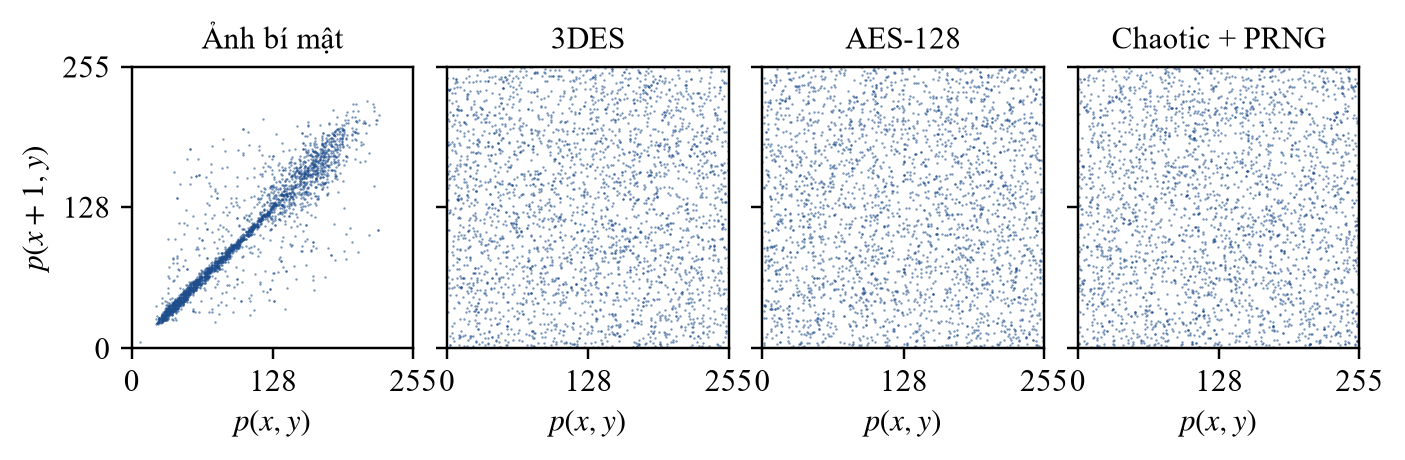
\includegraphics[width=\linewidth]{adjacent_scatter}
\caption{Phân bố cặp điểm ảnh kề theo chiều ngang (3000 cặp ngẫu nhiên)}
\label{fig:scatter}
\end{figure}

\subsection{Hiệu năng tốc độ mã hóa}

\bang{tab:enctime} và \hinh{fig:enctime} so sánh thời gian mã hóa với bài báo.

\begin{table}[H]
\centering
\caption{Thời gian mã hóa ($\mu$s) -- kịch bản B: 8000 lượt mỗi thuật toán}
\label{tab:enctime}
\small
\begin{tabular}{@{}lrrrrr@{}}
\toprule
\thead{Thuật toán} & \thead{Bài báo} & \thead{Trung bình} & \thead{Trung vị} & \thead{P95} & \thead{$246\times300$}\\
\midrule
3DES-192 CBC          & \num{3552} & \num{1303.1} & \num{1199.6} & \num{1602.2} & \num{3587.7}\\
AES-128 CBC           & 601        & 111.1        & 100.4        & 149.3        & 285.1\\
Chaotic + PRNG        & 36.2       & 31.3         & 26.0         & 51.3         & 834.5\textsuperscript{*}\\
\bottomrule
\multicolumn{6}{@{}l}{\footnotesize \textsuperscript{*} Không cache mặt nạ: thời gian gồm cả sinh \num{73800} giá trị Logistic và \num{73800} byte PRNG.}
\end{tabular}
\end{table}

\begin{figure}[H]
\centering
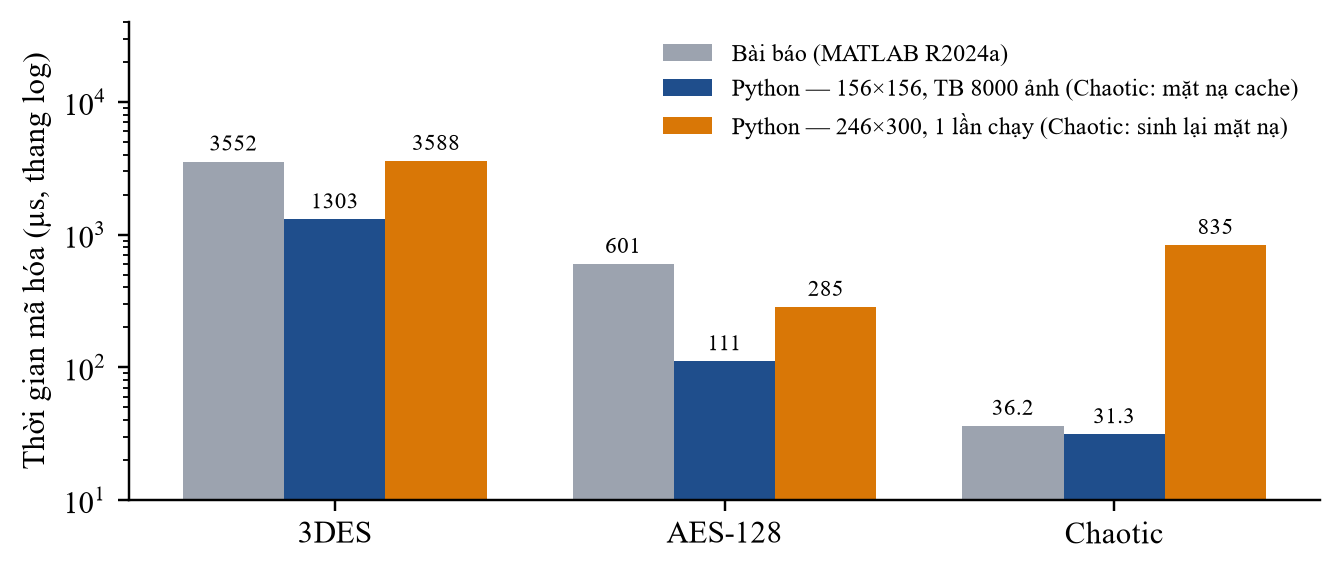
\includegraphics[width=0.9\linewidth]{enctime_compare}
\caption{Thời gian mã hóa: bài báo và kết quả tái hiện (thang logarit)}
\label{fig:enctime}
\end{figure}

\begin{figure}[H]
\centering
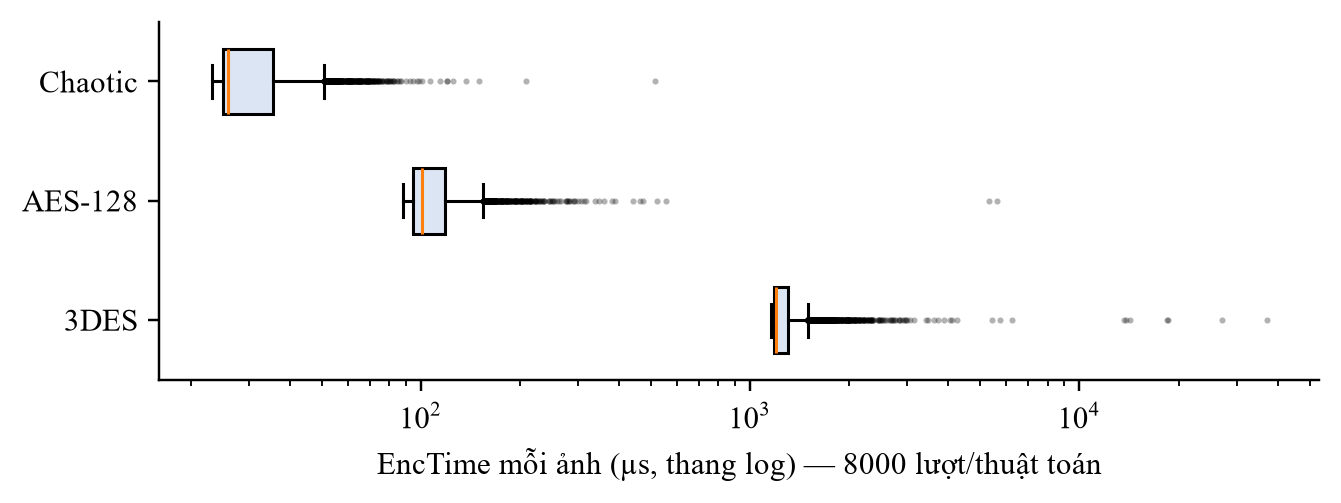
\includegraphics[width=0.9\linewidth]{enctime_distribution}
\caption{Phân bố thời gian mã hóa trên 8000 lượt chạy của mỗi thuật toán}
\label{fig:enctime-dist}
\end{figure}

Nhận xét:
\begin{itemize}
  \item Thứ tự tốc độ \textbf{Chaotic $<$ AES $<$ 3DES} của bài báo được tái hiện đúng. Với ảnh
        $156\times156$, Chaotic nhanh hơn 3DES khoảng $41.6$ lần và nhanh hơn AES khoảng $3.5$ lần;
        AES nhanh hơn 3DES khoảng $11.7$ lần.
  \item Thời gian 3DES trên ảnh $246\times300$ (\SI{3588}{\micro s}) gần như trùng giá trị
        \SI{3552}{\micro s} của bài báo. Điều này củng cố nhận định ở BM-01 rằng bài báo đo EncTime
        trên ảnh ``coins'' kích thước đầy đủ.
  \item AES trong bản tái hiện nhanh hơn bài báo khoảng $5.4$ lần nhờ PyCryptodome dùng tập lệnh
        phần cứng AES-NI. 3DES không có hỗ trợ phần cứng tương tự nên chậm hơn hẳn, vì phải chạy 48
        vòng Feistel trên khối 64 bit.
  \item Con số \SI{36.2}{\micro s} của Chaotic trong bài báo chỉ đạt được khi \emph{mặt nạ được tính
        sẵn} và chỉ đo phép XOR (chế độ cache: \SI{31.3}{\micro s}). Nếu tính cả chi phí sinh mặt nạ,
        Chaotic trên ảnh $246\times300$ mất \SI{834.5}{\micro s}, chậm hơn AES. Như vậy lợi thế tốc
        độ ``hai bậc độ lớn'' mà bài báo nêu phụ thuộc mạnh vào cách đo.
  \item Phân bố thời gian có đuôi dài (\hinh{fig:enctime-dist}) do ảnh hưởng của bộ lập lịch hệ điều
        hành và bộ nhớ đệm CPU; trung vị là đại lượng ổn định hơn trung bình khi so sánh.
\end{itemize}

\subsection{Phân tích theo lớp ảnh phủ}

Bài báo chỉ công bố giá trị trung bình gộp. Khi tách theo 5 lớp của Linnaeus 5
(\hinh{fig:class}), PSNR gần như không đổi nhưng SSIM và entropy ảnh stego khác nhau rõ rệt. Các
lớp nhiều kết cấu chi tiết như \code{dog} (SSIM $0.99721$, entropy $7.54$) và \code{berry}
($0.99709$; $7.51$) che giấu biến đổi LSB tốt hơn các lớp có nền phẳng như \code{flower}
($0.99653$) và \code{bird} ($0.99664$; entropy $7.37$). Nguyên nhân là SSIM nhạy với nhiễu $\pm1$
trên vùng phẳng hơn trên vùng nhiều chi tiết, gọi là hiệu ứng che lấp thị giác (\tn{visual
masking}). Kết quả trên tập \code{train} và \code{test} gần như trùng nhau (PSNR chênh dưới
\SI{0.001}{dB}, SSIM chênh dưới $0.0001$), cho thấy cỡ mẫu 8000 ảnh đủ để các giá trị trung bình
hội tụ.

\begin{figure}[H]
\centering
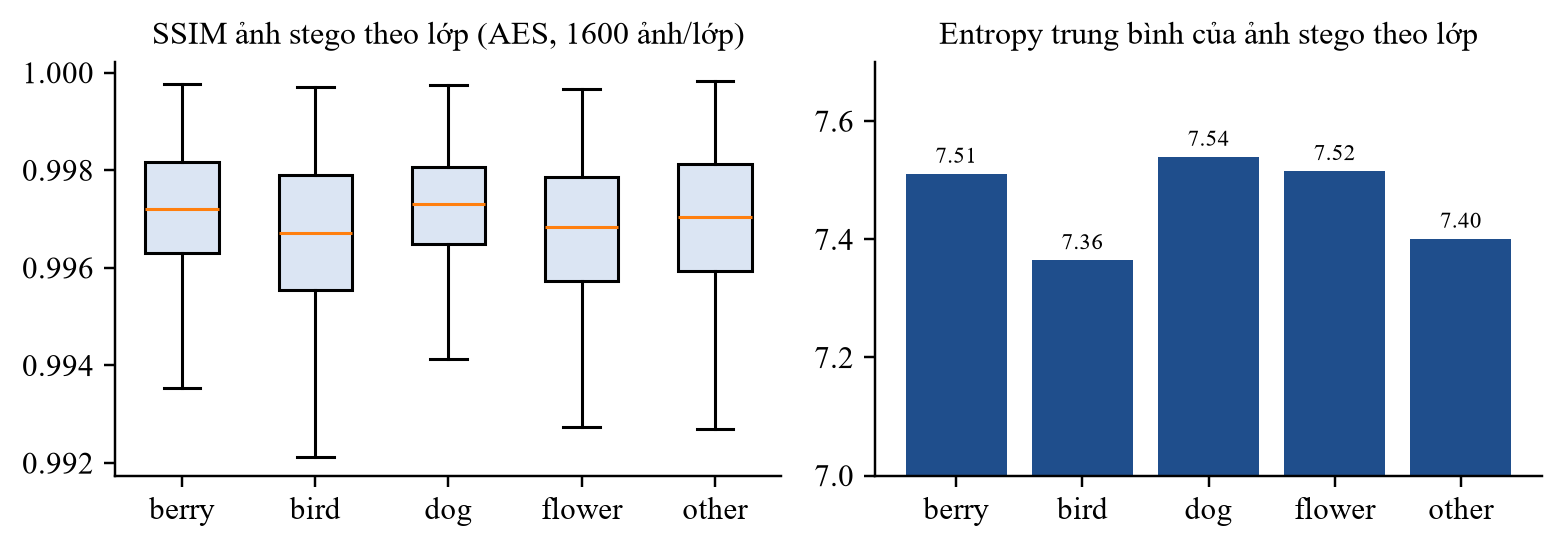
\includegraphics[width=\linewidth]{class_analysis}
\caption{SSIM và entropy ảnh stego theo 5 lớp ảnh phủ của Linnaeus 5}
\label{fig:class}
\end{figure}

\subsection{Đối chiếu tổng hợp với Bảng 2 của bài báo}

\bang{tab:compare-all} đặt cạnh nhau toàn bộ số liệu Bảng~2 của bài báo và kết quả tái hiện. Với
entropy, bản tái hiện đối chiếu cả hai cách đo.

\begin{table}[H]
\centering
\caption{Đối chiếu Bảng~2 của bài báo (BB) với kết quả tái hiện (TH) trên 8000 ảnh}
\label{tab:compare-all}
\footnotesize
\setlength{\tabcolsep}{4pt}
\begin{tabular}{@{}lrrrrrrl@{}}
\toprule
& \multicolumn{2}{c}{\thead{3DES}} & \multicolumn{2}{c}{\thead{AES-128}} & \multicolumn{2}{c}{\thead{Chaotic}} & \\
\cmidrule(lr){2-3}\cmidrule(lr){4-5}\cmidrule(lr){6-7}
\thead{Độ đo} & \thead{BB} & \thead{TH} & \thead{BB} & \thead{TH} & \thead{BB} & \thead{TH} & \thead{Mức khớp}\\
\midrule
MSE          & 0.49998 & 0.49560 & 0.50001 & 0.49577 & 0.49932 & 0.49544 & Rất sát\\
PSNR (dB)    & 51.1539 & 51.1795 & 51.1537 & 51.1780 & 51.1444 & 51.1809 & Rất sát\\
SSIM         & 0.99850 & 0.99686 & 0.99849 & 0.99686 & 0.99810 & 0.99686 & Sát\\
EncTime ($\mu$s) & 3552 & 1303 & 601 & 111 & 36.2 & 31.3 & Đúng thứ tự\\
NPCR (\%)    & 99.592 & 99.655 & 99.619 & 99.577 & 99.640 & 99.556 & Rất sát\\
UACI (\%)    & 30.808 & 30.325 & 30.818 & 30.348 & 30.961 & 30.512 & Sát, đúng thứ tự\\
Tương quan   & 0.0003 & 0.0062 & $-0.0041$ & $-0.0014$ & $-0.0098$ & $-0.0134$ & $\approx 0$\\
Entropy stego & 7.048 & 7.466 & 7.048 & 7.466 & 6.953 & 7.466 & Cùng đối tượng\\
Entropy bản mã & -- & 7.993 & -- & 7.992 & -- & 7.993 & Bài báo không đo\\
\bottomrule
\end{tabular}
\end{table}

Có thể kết luận bản tái hiện khớp với bài báo ở các điểm chính: MSE, PSNR, NPCR khớp gần như tuyệt
đối; UACI và SSIM khớp ở mức sát với chênh lệch đã được giải thích; thứ tự tốc độ được giữ nguyên.
Riêng entropy ảnh stego của bản tái hiện ($7.47$) cao hơn bài báo ($7.05$). Đây là đại lượng phụ
thuộc hoàn toàn vào ảnh phủ chứ không vào thuật toán, nên khác biệt có thể đến từ cách bài báo tính
entropy cho ảnh màu (ví dụ chuyển sang ảnh xám trước khi tính).

% =====================================================================
\section{Phân tích an toàn mở rộng}
\label{sec:antoan-morong}
% =====================================================================

Các độ đo trong bài báo chủ yếu mô tả \emph{tính thống kê} của bản mã và ảnh stego. Một hệ mật mã
chỉ có thể coi là an toàn khi chịu được các mô hình tấn công cụ thể. Phần này đánh giá thêm năm khía
cạnh mà bài báo chưa đề cập, dùng chính mã nguồn đã cài đặt và ảnh bí mật $156\times156$.

\subsection{Độ nhạy khóa}

Một hệ mật tốt phải cho bản mã khác hoàn toàn khi khóa thay đổi dù rất nhỏ, và giải mã bằng khóa
gần đúng không được tiết lộ thông tin. \bang{tab:keysens} cho thấy cả ba thuật toán đều đạt yêu cầu
này: đảo một bit khóa 3DES/AES, hay thay đổi $x_0$ hoặc $r$ chỉ $10^{-10}$, đều làm khoảng $99.3$--$99.6\%$
điểm ảnh bản mã thay đổi, UACI xấp xỉ $33.4\%$ (giá trị của hai ảnh ngẫu nhiên độc lập), và ảnh giải
mã bằng khóa sai chỉ còn là nhiễu (PSNR $\approx \SI{8.7}{dB}$). Với Chaotic, NPCR thấp hơn đôi chút
($99.3\%$) vì hai quỹ đạo Logistic chỉ tách nhau sau khoảng 30 bước lặp (\hinh{fig:logistic}b), nên
vài chục byte đầu của hai bản mã trùng nhau.

\begin{table}[H]
\centering
\caption{Độ nhạy khóa: so sánh bản mã của khóa đúng và khóa bị thay đổi rất nhỏ}
\label{tab:keysens}
\small
\begin{tabularx}{\linewidth}{@{}lLrrr@{}}
\toprule
\thead{Thuật toán} & \thead{Thay đổi khóa} & \thead{NPCR (\%)} & \thead{UACI (\%)} & \thead{PSNR giải mã sai}\\
\midrule
3DES    & Đảo 1 bit của $K_1$ (bit 1, byte 0) & 99.626 & 33.385 & \SI{8.61}{dB}\\
AES-128 & Đảo 1 bit của khóa (bit 0, byte 0)  & 99.552 & 33.466 & \SI{8.63}{dB}\\
Chaotic & $x_0 \to x_0 + 10^{-10}$            & 99.310 & 32.708 & \SI{8.72}{dB}\\
Chaotic & $r \to r + 10^{-10}$                & 99.240 & 32.771 & \SI{8.71}{dB}\\
Chaotic & \code{ecc\_seed}: $42 \to 43$       & 99.643 & 33.390 & \SI{8.72}{dB}\\
\bottomrule
\end{tabularx}
\end{table}

\subsection{Độ nhạy bản rõ -- phân tích vi sai đúng định nghĩa}

Trong phân tích vi sai chuẩn \cite{wu2011npcr}, kẻ tấn công mã hóa hai ảnh chỉ khác nhau \emph{một
điểm ảnh} rồi so sánh hai bản mã. Lược đồ tốt phải cho NPCR $\approx 99.6\%$ để không có quan hệ
khai thác được giữa thay đổi bản rõ và thay đổi bản mã. \bang{tab:plainsens} cho kết quả khi tăng
giá trị một điểm ảnh lên 1 ở ba vị trí khác nhau.

\begin{table}[H]
\centering
\caption{Độ nhạy bản rõ: NPCR/UACI (\%) giữa hai bản mã khi ảnh bí mật đổi đúng một điểm ảnh}
\label{tab:plainsens}
\small
\begin{tabular}{@{}lrrr@{}}
\toprule
\thead{Vị trí điểm ảnh thay đổi} & \thead{3DES} & \thead{AES-128} & \thead{Chaotic}\\
\midrule
Đầu ảnh $(0, 0)$        & 99.626 / 33.520 & 99.667 / 33.600 & 0.0041 / 0.00002\\
Giữa ảnh $(78, 78)$     & 49.511 / 16.594 & 49.466 / 16.483 & 0.0041 / 0.00005\\
Cuối ảnh $(155, 155)$   & 0.0329 / 0.0151 & 0.0657 / 0.0272 & 0.0041 / 0.00008\\
\bottomrule
\end{tabular}
\end{table}

Kết quả phản ánh đúng cấu trúc của từng thuật toán:
\begin{itemize}
  \item Với CBC, thay đổi ở khối $P_i$ lan sang mọi khối \emph{phía sau} theo \pt{eq:cbc}. Thay đổi
        điểm ảnh đầu làm toàn bộ bản mã thay đổi, ở giữa ảnh thì khoảng một nửa, còn ở điểm ảnh cuối
        thì chỉ đúng một khối thay đổi (8 byte $= 0.033\%$ với 3DES, 16 byte $= 0.066\%$ với AES).
  \item Với Chaotic + PRNG, dòng khóa không phụ thuộc bản rõ nên thay đổi một điểm ảnh chỉ làm
        \emph{đúng một byte} bản mã thay đổi ($1/\num{24336} = 0.0041\%$). Lược đồ hoàn toàn không có
        tính khuếch tán.
\end{itemize}
Như vậy, NPCR $\approx 99.6\%$ trong bài báo (đo giữa ảnh bí mật và bản mã) \emph{không} chứng minh
được khả năng chống tấn công vi sai. Khi đo đúng định nghĩa, Chaotic thất bại hoàn toàn, còn 3DES và
AES ở chế độ CBC với IV cố định chỉ đạt yêu cầu khi thay đổi nằm ở đầu ảnh.

\subsection{Tấn công biết bản rõ lên lớp Chaotic + PRNG}

Mặt nạ của lớp Chaotic được sinh từ các tham số cố định $(x_0, r, \mathit{seed})$, không phụ thuộc
bản rõ và không có số dùng một lần (\tn{nonce}). Vì vậy mọi ảnh đều được XOR với \emph{cùng một dòng
khóa} và lược đồ rơi vào đúng trường hợp dùng lại dòng khóa ở \pt{eq:twotime}. Em mô phỏng một kẻ tấn
công biết một cặp (ảnh bí mật $A$, bản mã $C_A$), ví dụ một ảnh đã từng bị lộ, và thu được bản mã
$C_B$ của một ảnh khác $B$ (ảnh ``camera''). Kết quả ở \hinh{fig:kpa}:
\begin{itemize}
  \item Chỉ cần XOR hai bản mã, $C_A \xor C_B = A \xor B$ đã lộ rõ đường nét chồng lên nhau của cả
        hai ảnh (hệ số tương quan với $A \xor B$ bằng $1.0$);
  \item Dòng khóa khôi phục được bằng $A \xor C_A$, từ đó giải mã được $B = C_B \xor (A \xor C_A)$
        \textbf{chính xác 100\%} mà không cần biết $x_0$, $r$ hay seed;
  \item Cùng phép tấn công đó với AES-CBC chỉ cho ra nhiễu (PSNR \SI{7.84}{dB}, tương quan $0.005$),
        vì AES là hoán vị giả ngẫu nhiên chứ không phải phép XOR với dòng khóa cố định.
\end{itemize}

\begin{figure}[H]
\centering
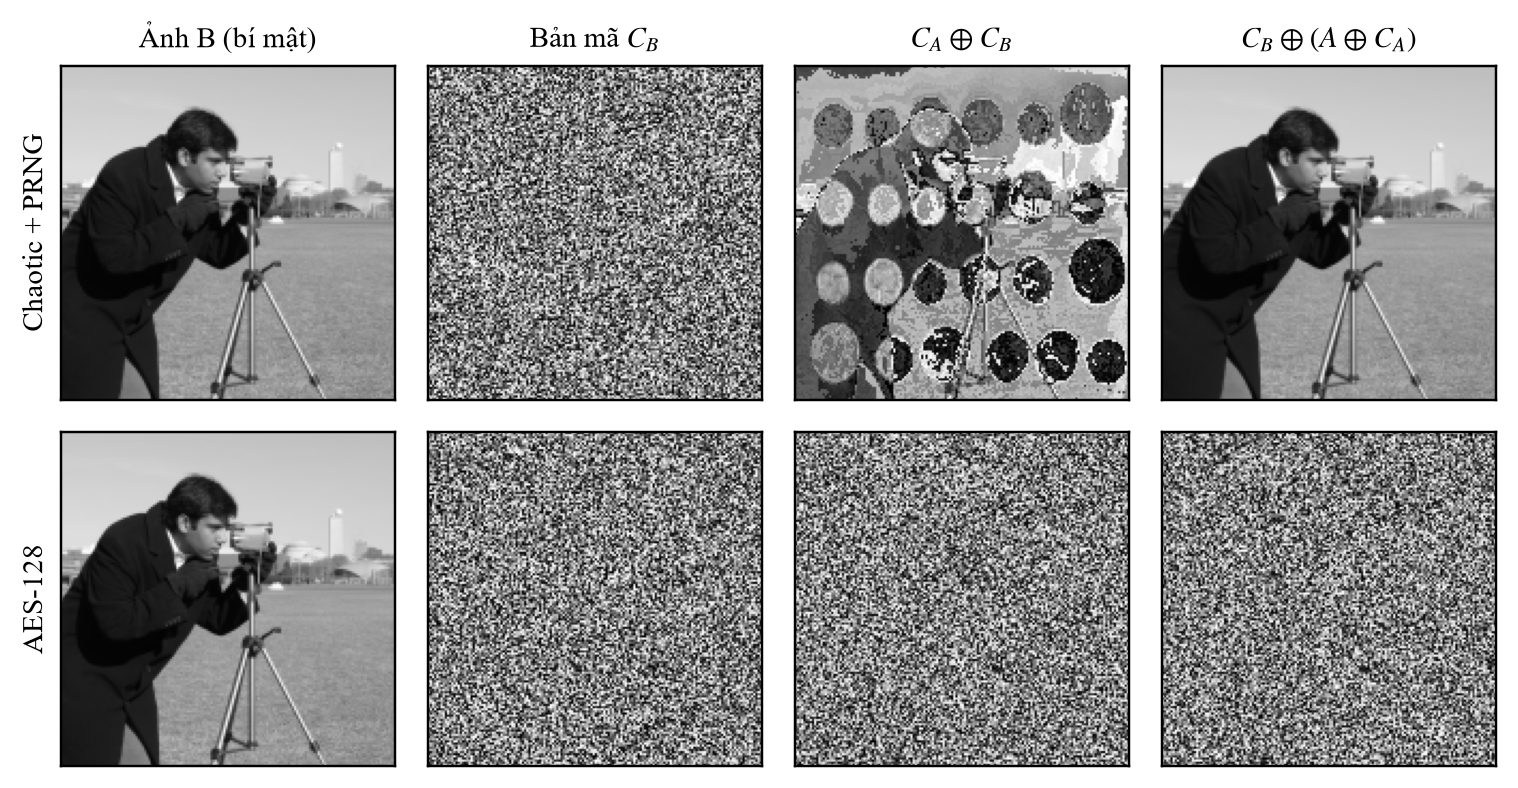
\includegraphics[width=0.95\linewidth]{kpa_attack}
\caption{Tấn công biết bản rõ: lớp Chaotic + PRNG bị phá hoàn toàn, AES-CBC không bị ảnh hưởng}
\label{fig:kpa}
\end{figure}

Ngoài ra, bài báo công bố công khai $x_0 = 0.785398$, $r = 3.999$, và mặt nạ ``ECC'' chỉ phụ thuộc
một seed số nguyên. Không gian khóa thực tế vì thế rất nhỏ so với 112 bit của 3DES hay 128 bit của
AES, vi phạm cả nguyên lý Kerckhoffs lẫn các yêu cầu cơ bản cho hệ mật hỗn loạn mà Alvarez và Li đã
nêu \cite{alvarez2006}. Kết luận rằng phương pháp hỗn loạn ``an toàn và nhanh hơn'' của bài báo vì
vậy cần được hiểu thận trọng: nó nhanh hơn chính vì nó chỉ là một mã dòng đơn giản dùng lại khóa.

\subsection{Khả năng chống chỉnh sửa}

Dùng phòng thí nghiệm tấn công của ứng dụng (Tab~2), em áp dụng năm kịch bản lên ảnh stego của cả ba
thuật toán. Kết quả tổng hợp ở \bang{tab:tamper} và \hinh{fig:tamper}.

\begin{table}[H]
\centering
\caption{Phản ứng của hệ thống trước các kịch bản tấn công/chỉnh sửa ảnh stego}
\label{tab:tamper}
\small
\begin{tabularx}{\linewidth}{@{}P{3.3cm}P{2.5cm}LL@{}}
\toprule
\thead{Kịch bản} & \thead{Dừng ở bước} & \thead{3DES / AES-128} & \thead{Chaotic}\\
\midrule
Không tấn công & -- & Khôi phục chính xác & Khôi phục chính xác\\
Giải mã sai khóa (seed + 1) & Giải mã & Phát hiện: lỗi gỡ đệm PKCS\#7; dữ liệu thô là nhiễu (PSNR 8.66/8.67 dB) & Không phát hiện: trả về ảnh nhiễu như kết quả hợp lệ (PSNR 8.72 dB)\\
Nén JPEG Q = 95 & Header & \multicolumn{2}{l}{Phát hiện: sai magic \code{HCST}, toàn bộ LSB bị phá hủy}\\
Đảo 1 bit trong header & Header & \multicolumn{2}{l}{Phát hiện: CRC-16 không khớp}\\
Đảo 1\% bit payload & Giải mã & Lỗi lan truyền theo khối: BER 24.1\% / 35.9\%, PSNR 11.9 / 10.0 dB; lần này lỗi đệm báo hiệu & Không phát hiện: BER đúng 1.0\%, PSNR 24.9 dB, lỗi rải rác\\
Nhiễu Gauss $\sigma = 2$ & Header & \multicolumn{2}{l}{Phát hiện: sai magic \code{HCST}}\\
\bottomrule
\end{tabularx}
\end{table}

\begin{figure}[H]
\centering
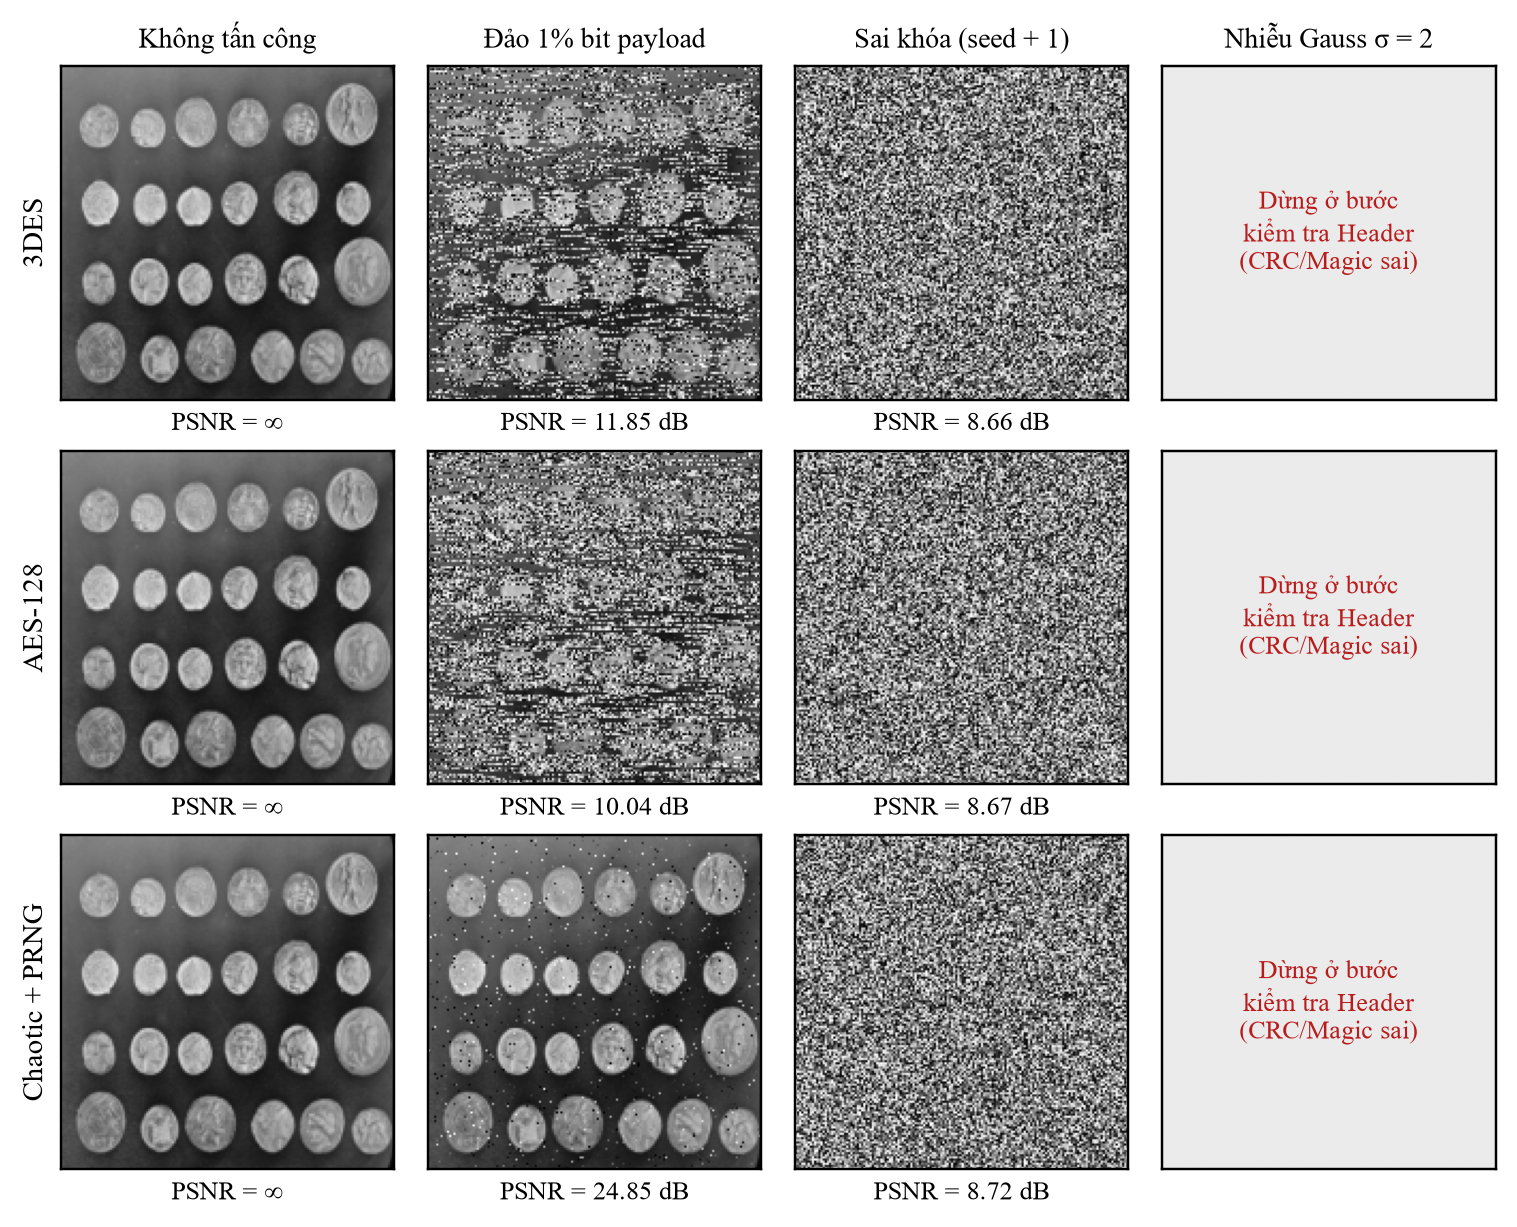
\includegraphics[width=0.92\linewidth]{tamper_grid}
\caption{Ảnh khôi phục dưới các kịch bản tấn công (cột cuối: bị chặn ngay ở bước kiểm tra header)}
\label{fig:tamper}
\end{figure}

Những nhận xét rút ra:
\begin{itemize}
  \item Giấu tin LSB thay thế là kỹ thuật \emph{mong manh} (\tn{fragile}): chỉ một lần nén JPEG chất
        lượng cao hoặc nhiễu rất nhỏ cũng phá hủy toàn bộ thông điệp. Header có magic và CRC-16 giúp
        hệ thống phát hiện ngay các trường hợp này thay vì giải mã ra dữ liệu rác, nhưng không khôi
        phục được thông điệp.
  \item CRC-16 chỉ phát hiện sai lệch ngẫu nhiên. Kẻ tấn công chủ động có thể sửa header rồi tính
        lại CRC. Phần payload hoàn toàn không được bảo vệ toàn vẹn: với 3DES/AES, việc phát hiện chỉ
        là ``tình cờ'' khi khối cuối bị hỏng làm sai đệm PKCS\#7; với Chaotic thì không có bất kỳ cơ
        chế phát hiện nào.
  \item Ở khía cạnh độ bền, Chaotic lại có ưu điểm: lỗi bit không lan truyền nên ảnh khôi phục vẫn
        nhận ra được (PSNR \SI{24.9}{dB}), trong khi CBC khuếch đại mỗi bit lỗi thành cả một khối
        hỏng.
\end{itemize}

\subsection{Khả năng bị phát hiện bởi phân tích giấu tin}

Mục tiêu cốt lõi của lớp giấu tin là không bị phát hiện. Tuy nhiên, ở chế độ 1-LSB lấp $99\%$ dung
lượng, mặt phẳng bit thấp nhất của ảnh stego bị thay hoàn toàn bằng dữ liệu ngẫu nhiên
(\hinh{fig:lsb-plane}). Trong khi đó mặt phẳng bit thấp của ảnh tự nhiên vẫn còn mang dấu vết cấu trúc
của ảnh, đặc biệt ở các vùng bão hòa hoặc phẳng.

\begin{figure}[H]
\centering
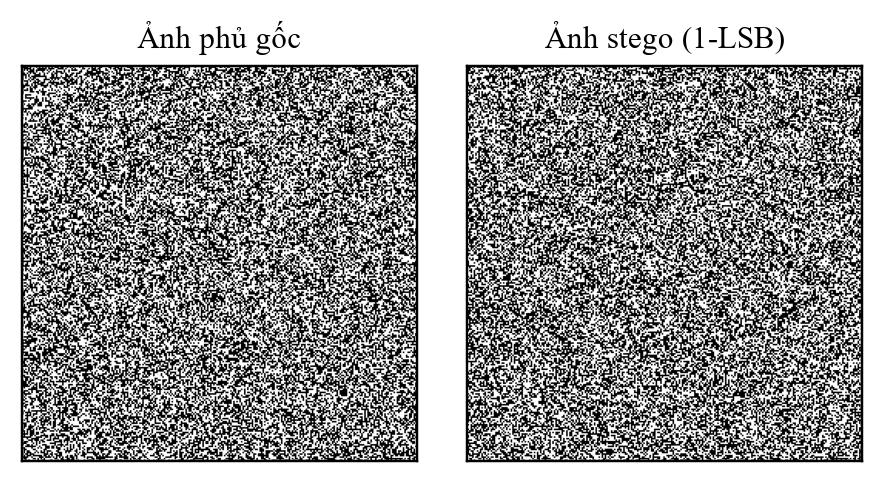
\includegraphics[width=0.62\linewidth]{lsb_plane}
\caption{Mặt phẳng bit thấp nhất (kênh R) của ảnh phủ và ảnh stego}
\label{fig:lsb-plane}
\end{figure}

Em áp dụng kiểm định $\chi^2$ trên cặp giá trị của Westfeld và Pfitzmann \cite{westfeld2000} cho cả
8000 ảnh phủ và 8000 ảnh stego tương ứng (AES, $156\times156$). Ảnh được coi là ``có giấu tin'' khi
giá trị $p > 0.95$. Kết quả (\hinh{fig:chi2}):
\begin{itemize}
  \item \textbf{99.84\%} ảnh stego bị phát hiện (trung vị $p = 0.999999$);
  \item chỉ \textbf{4.58\%} ảnh phủ gốc bị báo nhầm (trung vị $p \approx 2.4\times10^{-24}$).
\end{itemize}
Như vậy, với một phép kiểm định thống kê đơn giản công bố từ năm 1999, kẻ tấn công gần như luôn biết
ảnh nào đang mang tin. Lớp giấu tin của bài báo vì thế không đạt được mục tiêu ``vô hình'' trước một
đối thủ có kiến thức, dù đạt PSNR rất cao trước mắt người. Lý do là LSB \emph{thay thế} làm cân bằng
tần suất của các cặp giá trị $(2k, 2k+1)$, một dấu vết mà ảnh tự nhiên không có.

\begin{figure}[H]
\centering
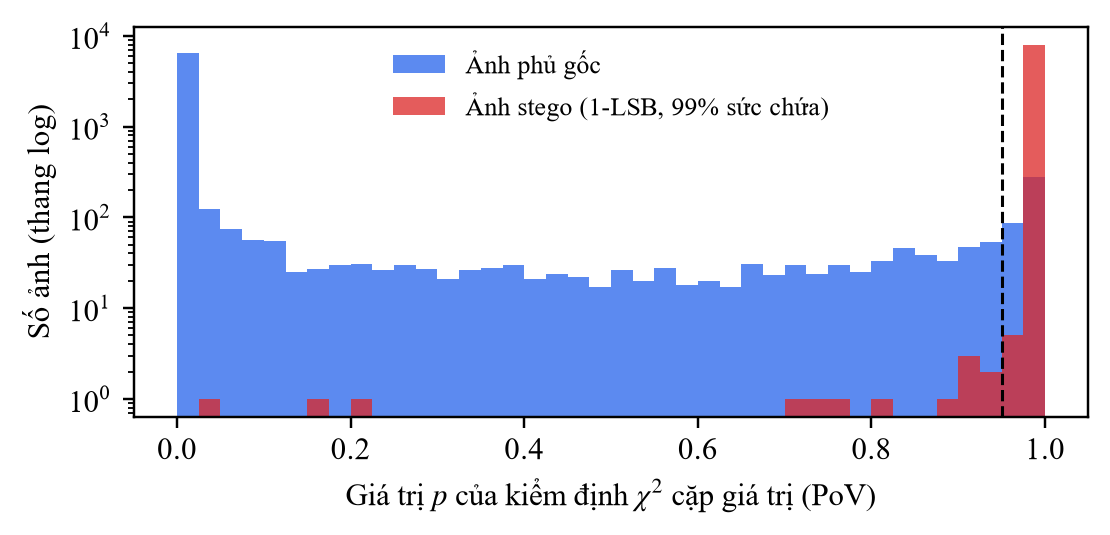
\includegraphics[width=0.82\linewidth]{chi2_steganalysis}
\caption{Phân bố giá trị $p$ của kiểm định $\chi^2$ cặp giá trị trên 8000 ảnh phủ và 8000 ảnh stego
(đường đứt: ngưỡng $p = 0.95$)}
\label{fig:chi2}
\end{figure}

\subsection{Tổng hợp đánh giá và đề xuất cải tiến}

\bang{tab:improve} tổng hợp các hạn chế đã được kiểm chứng bằng thực nghiệm và hướng khắc phục tương
ứng.

\begin{table}[H]
\centering
\caption{Các hạn chế đã kiểm chứng và đề xuất cải tiến}
\label{tab:improve}
\small
\begin{tabularx}{\linewidth}{@{}P{4.5cm}L@{}}
\toprule
\thead{Hạn chế} & \thead{Đề xuất khắc phục}\\
\midrule
Chaotic dùng lại dòng khóa; tham số công khai; không khuếch tán
  & Dẫn xuất dòng khóa từ khóa bí mật và một nonce ngẫu nhiên lưu trong header; tốt hơn là dùng mã dòng chuẩn như ChaCha20\\
IV cố định cho CBC: hai ảnh giống phần đầu cho bản mã giống phần đầu
  & Sinh IV ngẫu nhiên cho mỗi lần mã hóa và lưu vào header (IV không cần bí mật)\\
Không xác thực bản mã; CRC không chống sửa đổi có chủ đích
  & Dùng mã hóa có xác thực AES-GCM \cite{sp80038d} (hoặc ChaCha20-Poly1305) và đưa header vào dữ liệu liên kết (AAD) để mọi sửa đổi đều bị phát hiện\\
Khóa dẫn xuất từ seed công khai / SHA-256 của mật khẩu
  & Dùng hàm dẫn xuất khóa chậm có muối như Argon2 \cite{rfc9106} hoặc PBKDF2\\
3DES đã bị NIST loại bỏ, khối 64 bit dễ bị tấn công va chạm
  & Chỉ giữ 3DES để so sánh; dùng AES cho ứng dụng thực tế\\
LSB thay thế dễ bị kiểm định $\chi^2$ phát hiện
  & Dùng LSB matching ($\pm1$) \cite{mielikainen2006}, hoán vị vị trí nhúng bằng khóa, giảm tỷ lệ tải tin hoặc dùng giấu tin thích nghi \cite{holub2014}\\
Giấu tin không bền trước nén và nhiễu
  & Nếu cần độ bền: kết hợp mã sửa lỗi và nhúng trong miền biến đổi (DCT/DWT), chấp nhận giảm dung lượng\\
\bottomrule
\end{tabularx}
\end{table}

